\documentclass{article}

\usepackage{iclr2026_conference,times}
\input{math_commands.tex}

\usepackage{hyperref}
\hypersetup{
  colorlinks=false,
  pdfborder={0 0 1},
  citebordercolor={0 1 0},
  linkbordercolor={1 0 0},
  urlbordercolor={0 1 0}
}
\usepackage{url}
\usepackage{booktabs}
\usepackage{amsmath}
\usepackage{amssymb}
\usepackage{amsthm}
\usepackage{graphicx}
\usepackage{array}
\usepackage{longtable}

\newtheorem{definition}{Definition}
\newtheorem{proposition}{Proposition}
\newtheorem{lemma}{Lemma}

\title{Robotic Common Sense as Executable Affordance Tests}

\author{Anonymous Authors}

\begin{document}

\maketitle

\paragraph{Submission-hardening version: v3 final full-scale.}
This version replaces the compact v2 stress test with a multi-family
full-scale synthetic evaluation.  The new run covers 20 object categories, 10
affordance predicates, 8 deployment regimes, 10 mechanisms, 7 experiment
families, 192,000 main robot-object-task cases, 1,920,000 main method decisions,
and 4,977,600 aggregate method decisions overall.  The evidence remains
synthetic and mechanism-level: it does not claim real-robot validation.  The
central strengthened claim is that executable witnesses are useful when they
are selected with explicit cost, demand, and validity conditions; testing is
not a universal safety theorem.

\begin{abstract}
Robotic ``common sense'' is often treated as a prior over familiar facts: mugs
hold liquid, knives cut, sponges wipe, boxes support objects.  That framing is
fragile for embodied agents because deployment failures often preserve the name
while changing the physics: a mug leaks, a box is wet, a knife is dull, a tray
warps under heat, a gripper is weaker than expected, or the task demand exceeds
the familiar use case.  We propose Executable Affordance Test Logic (EATL), a
semantics in which a robotic common-sense predicate is not licensed by a text
fact, category label, or passive score alone, but by an executable
task-demand-specific witness for the current robot, object, action, and demand.
The witness can pass, fail, or abstain, and it carries a cost and a validity
scope.  We give simple bounds showing why label-only priors fail under
label-preserving affordance flips, when cost-aware testing is warranted, and
why stale witnesses become unsafe when their validity conditions are violated.
We then evaluate the mechanism in a transparent synthetic tabletop world.  In a
192,000-case main benchmark, the text prior has 0.188 unsafe false positives
under label-preserving flips and 0.197 under adversarial counterfeits; a
risk-aware EATL selector reduces those rates to 0.015 and 0.025 while using
less test cost than eager testing.  Phase diagrams, selector ablations, cache
validity tests, probe-noise sweeps, visibility ladders, demand shifts, and
failure galleries identify the boundary: when hidden flips are rare or probes
are expensive, conservative priors can dominate.  The contribution is therefore
not ``always test,'' but a precise operational semantics for when a robot may
assert embodied common sense.
\end{abstract}

\section{Introduction}

Robots inherit an attractive shortcut from language: if an object is called a
mug, use mug common sense.  That shortcut is often practical.  A robot should
not rediscover from scratch that a bowl can contain cereal, that a sponge can
wipe a spill, or that a brick can support weight.  Modern language-conditioned
robotics, affordance detectors, knowledge bases, and robot foundation models
all benefit from the fact that names and appearances are correlated with many
physical regularities.

The shortcut becomes dangerous when the name is stable but the relevant
physical predicate is not.  A mug can have a hole.  A cup-shaped sieve can be
concave but porous.  A knife can be decorative and dull.  A cardboard box can be
wet, crushed, or overloaded.  A plastic tray can look useful until the demanded
temperature changes.  A gripper with a weaker force limit may make an otherwise
reasonable lift predicate false.  These are not philosophical edge cases; they
are ordinary deployment changes in material, damage, wear, counterfeit objects,
task demand, and robot embodiment.

This paper argues that robotic common sense should be executable.  The claim
\texttt{can-contain-liquid(object, 350ml)} should mean that the robot has a
current witness for the relevant physical relation: a bounded diagnostic pour,
leak observation, stability check, and guard.  The claim
\texttt{can-support-load(object, 1kg)} should mean that the robot has a load
witness or a valid cached certificate under the current load demand.  The claim
\texttt{can-grasp-without-crushing(object, force)} should depend on the robot's
end effector and the object's crush limit, not merely on the object's name.

This reframing is intentionally narrower than general affordance learning.  It
does not claim that tests must be hand-written, that tests are free, or that
passive perception is useless.  It claims that an embodied common-sense
assertion is unsupported unless the robot has evidence that licenses the
assertion for the current robot-object-demand tuple.  That evidence may come
from a learned model, a tactile probe, a planner feasibility check, a cached
experiment, or a direct micro-action.  What matters is the semantics: the
predicate is tied to executable evidence, and lack of evidence is not the same
as truth.

The v2 version of this paper made the basic point with a small synthetic
experiment and a single test-cost stress.  The v3 version strengthens the
evidence and narrows the claim.  We evaluate a larger transparent environment
with 20 objects and 10 predicates, add risk-aware and cached variants, introduce
adversarial same-name counterfeits, vary probe cost and failure harm, examine
cache staleness, sweep sensor noise and guard design, give passive baselines
more hidden variables, and vary task demand and embodiment.  The result is more
useful and less absolute: executable witnesses can sharply reduce unsafe
assertions, but only if the robot accounts for test cost, failure harm,
abstention, and witness validity.

\paragraph{Contributions.}
First, we formalize Executable Affordance Test Logic (EATL): a common-sense
affordance predicate is licensed by a typed test program, observation trace,
guard, cost, and validity scope.  Second, we state simple formal results for
label-preserving flips, cost-aware testing, abstention, and stale witnesses.
Third, we provide a full-scale synthetic benchmark that attacks the mechanism
with stronger baselines, ablations, stress tests, and negative controls.  Fourth,
we document when EATL should lose: rare hidden flips, expensive probes,
incorrect cache reuse, high sensor noise, or passive visibility of the deciding
variable.

\section{Related Work and Novelty Boundary}

\paragraph{Affordances and action possibilities.}
Affordances originate as action possibilities relative to an actor
\citep{gibson1979ecological}; design work distinguishes perceived affordances
from physical constraints \citep{norman1988psychology}.  Robotics has long
modeled affordances as relations among objects, actions, and effects
\citep{sahin2007afford,montesano2008learning,stoytchev2005behavior}.
Interactive object learning and object-action complexes ground representation
in action outcomes \citep{fitzpatrick2003learning,kruger2011object}.  These
lines make generic affordance prediction non-novel.  The distinction here is
semantic: a robot common-sense predicate is not accepted because an affordance
classifier predicts it; it is accepted because the robot has executable evidence
for the current demand.

\paragraph{Visual and learned affordance detection.}
RGB-D activity models, part-based tool-affordance detectors, and deep
affordance segmentation methods infer likely functions from passive
observations \citep{koppula2013learning,myers2015affordance,do2018affordancenet}.
Knowledge representations encode object affordances for reasoning
\citep{zhu2014reasoning}.  These systems can be inputs to EATL.  A visual model
may propose which test to run, estimate a prior, or sometimes directly observe
the deciding variable.  The novelty claim does not require passive perception
to fail.  It requires the paper to separate \emph{prediction} from
\emph{licensed assertion}: when the deciding variable is hidden, stale, or
demand-specific, a passive score is not itself a witness.

\paragraph{Planning and feasibility checking.}
Task-and-motion planning integrates symbolic choices with continuous
feasibility checks \citep{kaelbling2011hierarchical,toussaint2015logic,garrett2020pddlstream}.
This makes feasibility checks inside a planner non-novel.  EATL differs in
where the assertion lives.  It treats an embodied common-sense predicate as a
first-class object before plan execution: the predicate can pass, fail, abstain,
or expire, and that status can be reused by a planner or by a language
conditioned policy.  A failed pour probe is not just a low planning score; it is
a local failure certificate for a named physical relation.

\paragraph{Language-conditioned robotics and robot foundation models.}
Language models and multimodal models guide skill selection, planning, and
manipulation \citep{ahn2022saycan,huang2022inner,liang2023code,huang2023voxposer,driess2023palme,brohan2022rt1,brohan2023rt2,openx2023,shridhar2022cliport}.
Other work shows limitations of language-only planning
\citep{huang2022zeroshot,valmeekam2023plan}.  EATL is not an alternative to
foundation models.  It is a contract that such systems can satisfy or violate:
if a language-conditioned policy asserts that a mug can safely carry hot
liquid, the assertion should be tied to a witness for the current mug, robot,
and temperature, or explicitly marked as unsupported.

\paragraph{Interactive perception and world models.}
Robots can learn by poking, grasping, and predicting future observations
\citep{agrawal2016poke,pinto2016supersizing,ha2018world}.  EATL can use learned
world models as implementations of tests.  The proposed contribution is not
that interaction is useful; that is well established.  The contribution is that
robot common-sense predicates should be defined by the executable evidence that
would make them true for the current task.  This is a small but consequential
shift: the output is not only a policy or prediction, but a typed witness or
failure certificate.

\section{Executable Affordance Test Logic}

Let $o$ be an object instance, $r$ a robot embodiment, $a$ an action family, and
$d$ a task demand.  A conventional prior estimates $p(y \mid \ell, x)$, where
$\ell$ is an object label and $x$ is a passive observation.  EATL instead
attaches a test program to the predicate itself.

\begin{definition}[Executable affordance test]
For predicate $\phi$, an executable affordance test is a tuple
$T_{\phi}=(\pi_{\phi}, h_{\phi}, g_{\phi}, c_{\phi}, v_{\phi})$.  The
micro-policy $\pi_{\phi}$ chooses a bounded diagnostic action for
$(r,o,a,d)$.  The observation map $h_{\phi}$ returns a trace $\tau$.  The guard
$g_{\phi}(\tau)$ returns \textsc{pass}, \textsc{fail}, or \textsc{abstain}.
The scalar $c_{\phi}$ is the normalized cost of the test.  The validity
predicate $v_{\phi}$ specifies when the witness remains applicable.
\end{definition}

\begin{definition}[Witness and certificate]
The robot may assert $\phi(r,o,a,d)$ only if it has a witness
$(T_{\phi},\tau)$ such that $g_{\phi}(\tau)=\textsc{pass}$ and
$v_{\phi}(r,o,a,d,\tau)=1$.  If $g_{\phi}(\tau)=\textsc{fail}$, the trace is a
failure certificate.  If $g_{\phi}(\tau)=\textsc{abstain}$, the predicate is
unavailable for safe assertion.
\end{definition}

\begin{definition}[Cached witness]
A cached witness for $\phi$ is a previous pass trace with a stored validity
scope over object state, robot embodiment, task demand, and time.  Reuse is
licensed only if the current tuple lies inside that scope.  Label-only reuse is
not a valid cache policy unless the label is known to determine the predicate.
\end{definition}

Examples are deliberately mundane.  \texttt{can-contain-liquid} can be tested
by a safe pour probe that observes leakage and stability.  \texttt{can-lift}
can use a bounded lift and slip observation.  \texttt{can-support-load} can use
a calibration load below the task demand.  \texttt{can-cut-soft-food} can use a
low-force edge probe.  \texttt{can-wipe-spill} can measure absorption.
\texttt{can-carry-hot} can check heat resistance and handle availability.
\texttt{can-grasp-without-crushing} can test whether a required grip force
exceeds a fragile object's crush limit.  These are not full task rollouts.  They
are targeted micro-experiments whose observations address variables that names
or passive images may miss.

\section{Simple Formal Analysis}

The analysis is intentionally modest.  It does not prove that any particular
test implementation is safe.  It shows why labels are insufficient under a
specific hostile distribution, why cost-aware selection is required, and why
cached witnesses must carry validity conditions.

\begin{proposition}[Label-only error under affordance flips]
Fix an object label $\ell$ and binary affordance predicate $Y$.  Any classifier
$h$ that depends only on $\ell$ has conditional error
\[
  \Pr[h(\ell)\neq Y \mid L=\ell] \geq \min(p_{\ell},1-p_{\ell}),
\]
where $p_{\ell}=\Pr[Y=1\mid L=\ell]$.  If a deployment distribution presents
balanced same-label counterexamples, $p_{\ell}=1/2$, the error is at least
$1/2$.
\end{proposition}

\textit{Proof.}
For a fixed label, $h(\ell)$ is constant.  If it predicts 1, its error is
$1-p_{\ell}$; if it predicts 0, its error is $p_{\ell}$.  The better constant
choice therefore has error $\min(p_{\ell},1-p_{\ell})$.

\begin{proposition}[Test value threshold]
Suppose a prior policy would assert a predicate with estimated false-positive
probability $q$, false-positive harm $H$, and no test cost.  A test with
expected post-test false-positive probability $q_T$ and cost $C_T$ improves
expected safety-plus-test cost whenever
\[
  (q-q_T)H > C_T .
\]
If the inequality is reversed, eager testing is dominated by the prior for that
case.
\end{proposition}

\textit{Interpretation.}
This is the paper's core boundary.  EATL is not ``always test.''  It says the
robot should treat an affordance assertion as requiring executable evidence,
but obtaining evidence has cost.  A risk-aware selector should run a test when
the expected reduction in unsafe assertion harm exceeds probe cost, and abstain
or use a conservative prior otherwise.

\begin{proposition}[Abstention is not failure]
Let $\bot$ denote abstention.  If a policy returns $\bot$ whenever the expected
cost of both assertion and rejection exceeds an application-specific escalation
cost $C_{\bot}$, then abstention is preferable to forced assertion whenever
$qH > C_{\bot}$ and preferable to forced rejection whenever $pM>C_{\bot}$,
where $p$ is the probability the predicate is true and $M$ is the missed
opportunity or recovery cost.
\end{proposition}

The experiments use abstention conservatively, mostly in the conservative prior
and high-noise guard settings.  The proposition matters because a robot
common-sense system should be allowed to say ``unsupported'' rather than
hallucinating a safe physical fact.

\begin{proposition}[Invalid cache reuse]
Let a cached witness have original tuple $z=(r,o,a,d)$ and current tuple
$z'=(r',o',a,d')$.  If the cache policy reuses the witness whenever labels
match, but there exists a hidden variable $u$ such that
$\phi(z,u)=1$ and $\phi(z',u')=0$, then the cache policy has a positive unsafe
false-positive rate on any distribution assigning positive probability to
$(z,u,z',u')$.
\end{proposition}

This proposition is nearly tautological, but it exposes a common engineering
mistake.  A successful past test is useful only if the validity scope includes
the current robot, object state, and demand.  The v3 cache experiment quantifies
the mistake: label-only cache reuse has 0.270 unsafe false positives, while
strict validity reuse has 0.025 with lower cost than no cache.

\section{Synthetic Environment}

The environment is transparent by design.  It is not a photorealistic simulator
and not a hardware claim.  Each object has a name and hidden physical variables:
concavity, porosity, holes, capacity, mass, friction, load capacity, sharpness,
edge stiffness, absorbency, heat resistance, handle availability, base
stability, flatness, pour lip, crush limit, grippability, surface fragility, and
wetness.  Ground-truth affordances are deterministic functions of those
variables, task demands, and robot embodiment.

\paragraph{Objects.}
The v3 catalog contains 20 named categories: mug, bowl, sieve, knife, spoon,
sponge, brick, cardboard box, plastic tray, glass, thermos, paper cup, ceramic
plate, towel, wooden block, foam block, metal pan, silicone mat, mesh bag, and
rubber grip pad.  The names intentionally include ordinary household objects,
fragile objects, porous objects, heat-sensitive objects, and objects whose
visual geometry can be misleading.

\paragraph{Predicates.}
The ten task predicates are containment, lift, support load, cut soft food, wipe
spill, carry hot object, pour without spill, stack safely, push without sliding,
and grasp without crushing.  Each predicate is evaluated under a demand such as
volume, load, temperature, required sharpness, push force, or grip force.

\paragraph{Regimes.}
The main benchmark includes eight deployment regimes:
\textbf{typical}, with mild wear;
\textbf{label-preserving flips}, where hidden variables change while names do
not;
\textbf{label swaps}, where physical state is borrowed from another category;
\textbf{mixed}, which samples the previous regimes;
\textbf{adversarial counterfeits}, where a same-name object is modified to
break a high-confidence prior;
\textbf{degraded/worn}, with broad capacity and material degradation;
\textbf{task-demand shift}, where the demanded volume, load, temperature, or
force changes; and
\textbf{embodiment shift}, where the robot gripper or heat tolerance changes.

\paragraph{Methods.}
We compare ten mechanisms.  \textbf{text prior} uses object names only.
\textbf{calibrated text prior} weakens label confidence in hostile regimes.
\textbf{passive vision proxy} sees geometry-like variables but misses many
hidden material and damage variables.  \textbf{uncertainty vision proxy}
abstains near its decision boundary.  \textbf{conservative prior} asserts only
low-consequence high-confidence positives and otherwise rejects or abstains.
\textbf{eager EATL} always runs the predicate-specific test.
\textbf{risk-aware EATL} blends label and visible priors, estimates test value,
and runs tests when expected harm reduction exceeds test cost.
\textbf{cached EATL} reuses strict current-state witnesses when available.
\textbf{oracle hidden state} is an upper bound.  \textbf{random test control}
is an intentionally irrelevant negative control.

\paragraph{Metrics.}
The main safety metric is unsafe false-positive rate: cases where a method
asserts an affordance that is false.  We also report accuracy, avoidable false
negatives, abstention rate, F1, mean test cost, and mean total cost.  Total cost
adds test cost, false-positive harm, and a small false-negative recovery cost.
The absolute units are synthetic; the comparisons are meaningful because all
methods share the same cost accounting.

\section{Full-Scale Experiment Program}

The v3 runner executes seven aggregate experiment families and a bounded failure
gallery.  It avoids retaining full raw logs in memory: each family streams
through cases, keeps keyed counters, and writes aggregate CSVs.  The main family
uses 12 seeds, 8 regimes, 10 episodes per regime, 20 objects, 10 tasks, and 10
methods, for 192,000 robot-object-task cases and 1,920,000 method decisions.
The full suite writes 4,977,600 aggregate method decisions across main, phase,
selector, cache, noise, visibility, and demand/embodiment families.

Family A is the main multi-seed benchmark.  Family B sweeps hidden-flip rate,
test-harm weight, and failure harm to build a cost phase diagram.  Family C
ablates the risk-aware selector against eager testing, cheapest-test selection,
no failure-harm accounting, no test-harm accounting, no abstention, and random
testing.  Family D studies witness caches under object drift.  Family E sweeps
probe noise and guard design.  Family F gives passive perception progressively
more visibility into hidden variables.  Family G sweeps task demands and robot
embodiments.  Family H records representative failures, abstentions, saved
tests, and negative-control errors.

\section{Main Results}

Figure~\ref{fig:unsafe} and Table~\ref{tab:main} show the central result.  The
text prior is excellent in the typical regime because the catalog's names match
their ordinary physics: 0.994 accuracy and 0.004 unsafe false positives.  That
success is exactly why the shortcut is tempting.  Under label-preserving flips,
however, the text prior has 0.188 unsafe false positives and the passive proxy
has 0.212.  Eager EATL reduces the rate to 0.022, and risk-aware EATL reduces it
further to 0.015 while using lower mean test cost.  Under adversarial
counterfeits, the text prior has 0.197 unsafe false positives, passive vision
has 0.240, eager EATL has 0.037, and risk-aware EATL has 0.025.

\begin{figure}[t]
\centering
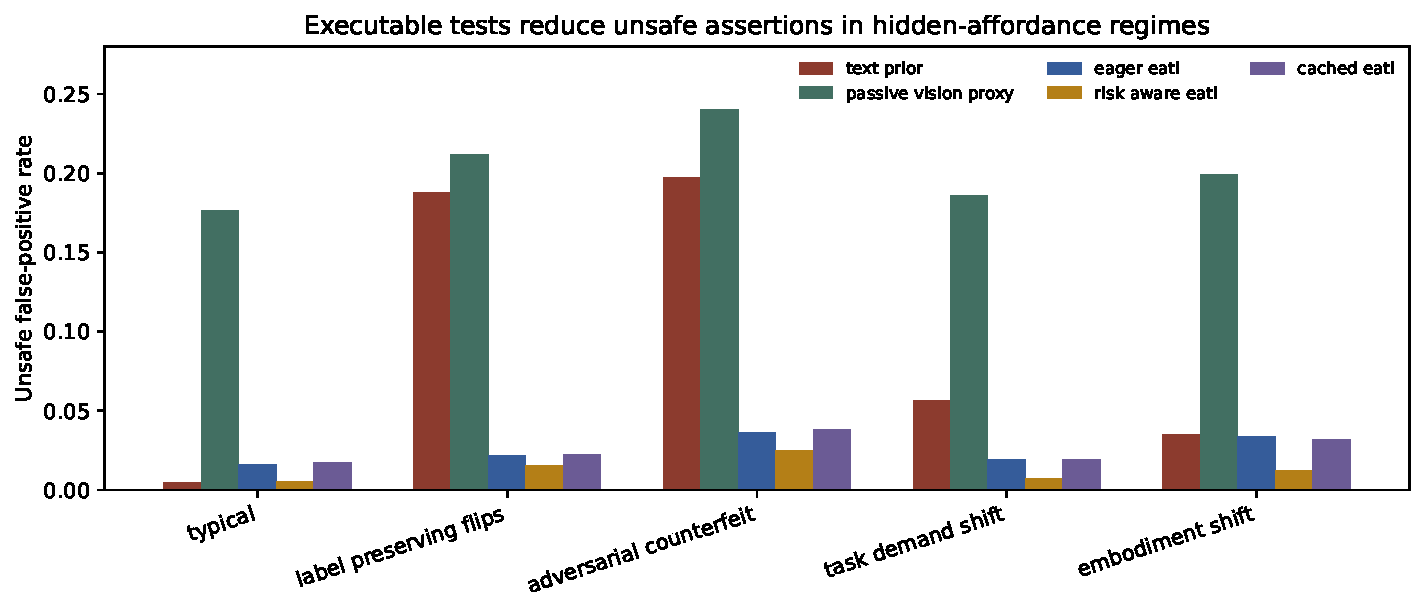
\includegraphics[width=\linewidth]{../figures/full_scale/unsafe_fp_by_regime.pdf}
\caption{Unsafe false-positive rates in the main v3 benchmark.  Name priors are
excellent on typical objects but break under hidden physical changes.  Eager and
risk-aware EATL reduce unsafe assertions; risk-aware EATL pays less test cost by
using prior and visible evidence when the test value is low.}
\label{fig:unsafe}
\end{figure}

\begin{table}[t]
\centering
\small
\resizebox{\linewidth}{!}{\begin{tabular}{llrrrrr}
\toprule
Regime & Method & Acc. & Unsafe FP & Abstain & Test cost & Total cost \\
\midrule
typical & text\_prior & 0.993 & 0.005 & 0.000 & 0.000 & 0.024 \\
 & passive\_vision\_proxy & 0.824 & 0.176 & 0.000 & 0.000 & 0.882 \\
 & conservative\_prior & 0.848 & 0.005 & 0.145 & 0.000 & 0.046 \\
 & eager\_eatl & 0.975 & 0.017 & 0.000 & 0.102 & 0.190 \\
 & risk\_aware\_eatl & 0.986 & 0.006 & 0.000 & 0.056 & 0.090 \\
 & cached\_eatl & 0.974 & 0.018 & 0.000 & 0.102 & 0.195 \\
 & oracle\_hidden\_state & 1.000 & 0.000 & 0.000 & 0.000 & 0.000 \\
\midrule
label\_preserving\_flips & text\_prior & 0.806 & 0.192 & 0.000 & 0.000 & 0.961 \\
 & passive\_vision\_proxy & 0.789 & 0.211 & 0.000 & 0.000 & 1.054 \\
 & conservative\_prior & 0.736 & 0.117 & 0.145 & 0.000 & 0.606 \\
 & eager\_eatl & 0.975 & 0.022 & 0.000 & 0.102 & 0.214 \\
 & risk\_aware\_eatl & 0.982 & 0.015 & 0.000 & 0.070 & 0.146 \\
 & cached\_eatl & 0.974 & 0.023 & 0.000 & 0.100 & 0.216 \\
 & oracle\_hidden\_state & 1.000 & 0.000 & 0.000 & 0.000 & 0.000 \\
\midrule
adversarial\_counterfeit & text\_prior & 0.802 & 0.196 & 0.000 & 0.000 & 0.980 \\
 & passive\_vision\_proxy & 0.761 & 0.239 & 0.000 & 0.000 & 1.197 \\
 & conservative\_prior & 0.740 & 0.113 & 0.145 & 0.000 & 0.588 \\
 & eager\_eatl & 0.957 & 0.037 & 0.000 & 0.102 & 0.293 \\
 & risk\_aware\_eatl & 0.968 & 0.027 & 0.000 & 0.078 & 0.214 \\
 & cached\_eatl & 0.960 & 0.035 & 0.000 & 0.083 & 0.261 \\
 & oracle\_hidden\_state & 1.000 & 0.000 & 0.000 & 0.000 & 0.000 \\
\midrule
task\_demand\_shift & text\_prior & 0.923 & 0.056 & 0.000 & 0.000 & 0.294 \\
 & passive\_vision\_proxy & 0.813 & 0.187 & 0.000 & 0.000 & 0.934 \\
 & conservative\_prior & 0.816 & 0.018 & 0.145 & 0.000 & 0.122 \\
 & eager\_eatl & 0.974 & 0.019 & 0.000 & 0.106 & 0.203 \\
 & risk\_aware\_eatl & 0.985 & 0.007 & 0.000 & 0.057 & 0.095 \\
 & cached\_eatl & 0.974 & 0.018 & 0.000 & 0.105 & 0.202 \\
 & oracle\_hidden\_state & 1.000 & 0.000 & 0.000 & 0.000 & 0.000 \\
\midrule
embodiment\_shift & text\_prior & 0.961 & 0.036 & 0.000 & 0.000 & 0.183 \\
 & passive\_vision\_proxy & 0.800 & 0.200 & 0.000 & 0.000 & 1.000 \\
 & conservative\_prior & 0.838 & 0.015 & 0.145 & 0.000 & 0.098 \\
 & eager\_eatl & 0.954 & 0.033 & 0.000 & 0.102 & 0.273 \\
 & risk\_aware\_eatl & 0.974 & 0.013 & 0.000 & 0.056 & 0.128 \\
 & cached\_eatl & 0.954 & 0.033 & 0.000 & 0.102 & 0.273 \\
 & oracle\_hidden\_state & 1.000 & 0.000 & 0.000 & 0.000 & 0.000 \\
\bottomrule
\end{tabular}
}
\caption{Main benchmark summary over 192,000 robot-object-task cases and
1,920,000 method decisions.  Total cost includes unsafe false positives, missed
true affordances, abstentions, and test cost under the shared synthetic cost
model.}
\label{tab:main}
\end{table}

The strongest positive finding is not merely that tests help; it is that
selective tests help more than eager tests.  In label-preserving flips, eager
EATL has mean total cost 0.213, while risk-aware EATL has 0.150.  In the mixed
regime, eager EATL has 0.202 total cost and risk-aware EATL has 0.109.  In
task-demand shift, risk-aware EATL achieves 0.985 accuracy and 0.007 unsafe
false positives, compared with 0.922 accuracy and 0.057 unsafe false positives
for the text prior.  This supports the v3 claim: the semantic shift to
executable witnesses should be paired with a policy that decides when evidence
is worth obtaining.

The main negative finding is equally important.  In the typical regime, the
text prior has lower total cost than risk-aware EATL because hidden flips are
rare and tests add overhead.  A conservative prior also has low unsafe risk in
some regimes by abstaining.  Therefore EATL should not be deployed as an
unconditional reflex.  It should be a licensing rule for assertion plus a
cost-aware procedure for obtaining or reusing evidence.

\section{Cost Phase Diagram}

The v2 paper reported one break-even test-harm value.  The v3 phase diagram
sweeps hidden-flip rate, test-harm weight, and failure harm.  At failure harm 5
and test-harm weight 1, Figure~\ref{fig:phase} shows that text priors dominate
when hidden flips are absent, but risk-aware testing becomes better as the flip
rate grows.  The table makes the boundary more precise.  At flip rate 0.10 and
test-harm weight 3, the text prior or conservative prior can win.  At flip rate
0.25, risk-aware EATL wins for moderate test costs and begins to lose only at
the highest test-harm settings.  At flip rate 0.75, risk-aware EATL wins across
all listed test costs because the unsafe-assertion harm dominates.

\begin{figure}[t]
\centering
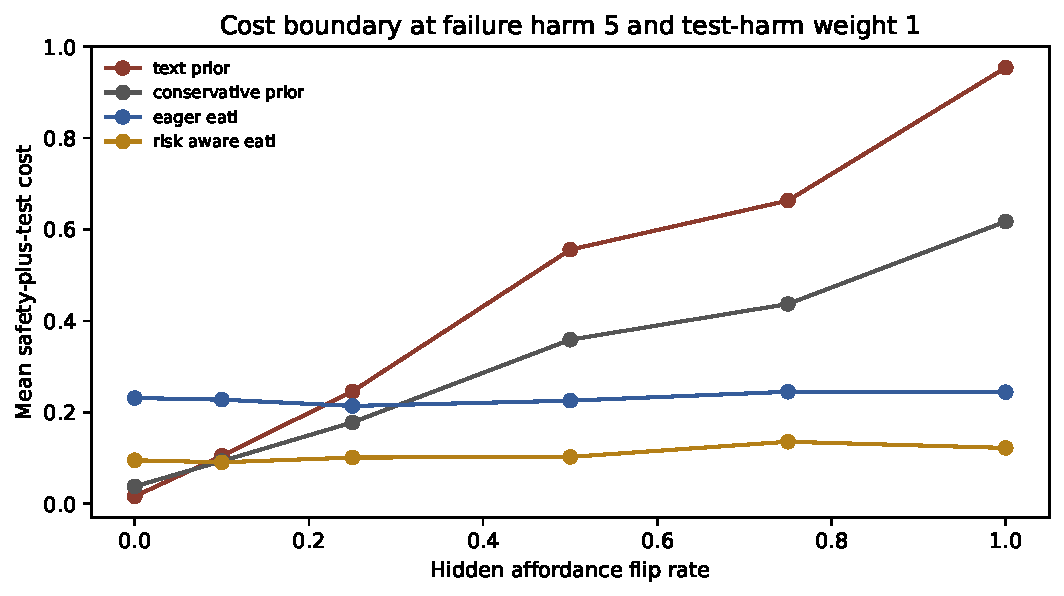
\includegraphics[width=0.82\linewidth]{../figures/full_scale/phase_hidden_rate_cost.pdf}
\caption{Cost phase diagram slice.  When hidden affordance flips are rare,
testing can be unnecessary overhead.  As the same-label flip rate rises,
risk-aware testing becomes the lowest-cost policy.}
\label{fig:phase}
\end{figure}

\begin{table}[t]
\centering
\scriptsize
\resizebox{\linewidth}{!}{\begin{tabular}{rrrrlrr}
\toprule
Flip rate & Test harm & Failure harm & Best & Risk-text & Eager-text & Text cost \\
\midrule
0.10 & 0.25 & 5.0 & risk\_aware\_eatl & -0.023 & 0.056 & 0.073 \\
0.10 & 0.25 & 10.0 & risk\_aware\_eatl & -0.041 & 0.114 & 0.145 \\
0.10 & 1.00 & 5.0 & conservative\_prior & 0.014 & 0.127 & 0.086 \\
0.10 & 1.00 & 10.0 & conservative\_prior & -0.016 & 0.144 & 0.171 \\
0.10 & 2.50 & 5.0 & conservative\_prior & 0.092 & 0.263 & 0.093 \\
0.10 & 2.50 & 10.0 & conservative\_prior & 0.041 & 0.308 & 0.184 \\
0.35 & 0.25 & 5.0 & risk\_aware\_eatl & -0.303 & -0.245 & 0.370 \\
0.35 & 0.25 & 10.0 & risk\_aware\_eatl & -0.625 & -0.495 & 0.738 \\
0.35 & 1.00 & 5.0 & risk\_aware\_eatl & -0.241 & -0.133 & 0.343 \\
0.35 & 1.00 & 10.0 & risk\_aware\_eatl & -0.548 & -0.334 & 0.686 \\
0.35 & 2.50 & 5.0 & risk\_aware\_eatl & -0.139 & 0.047 & 0.326 \\
0.35 & 2.50 & 10.0 & risk\_aware\_eatl & -0.447 & -0.169 & 0.651 \\
0.70 & 0.25 & 5.0 & risk\_aware\_eatl & -0.602 & -0.524 & 0.673 \\
0.70 & 0.25 & 10.0 & risk\_aware\_eatl & -1.239 & -1.057 & 1.344 \\
0.70 & 1.00 & 5.0 & risk\_aware\_eatl & -0.545 & -0.420 & 0.657 \\
0.70 & 1.00 & 10.0 & risk\_aware\_eatl & -1.144 & -0.945 & 1.312 \\
0.70 & 2.50 & 5.0 & risk\_aware\_eatl & -0.462 & -0.290 & 0.662 \\
0.70 & 2.50 & 10.0 & risk\_aware\_eatl & -1.085 & -0.808 & 1.323 \\
\bottomrule
\end{tabular}
}
\caption{Selected phase-boundary rows.  Negative Risk-text values mean
risk-aware EATL has lower total cost than the text prior.}
\label{tab:phase}
\end{table}

This result is a useful guard against overclaiming.  The paper's thesis is not
that every robot should test every object before every action.  The thesis is
that a robot should know whether an affordance assertion is licensed by current
evidence.  If the expected value of evidence is low, the system can reuse a
valid witness, use a conservative prior, abstain, or continue with a label prior
under explicit risk.

\section{Selector Ablations}

Table~\ref{tab:ablation} compares risk-aware EATL with policies that ignore
pieces of the selection problem.  The random test control is intentionally bad:
it pays test cost and still has unsafe false positives above 0.43 in the hostile
regimes.  Cheapest-test selection improves on the random control but remains
unsafe because cheap probes are not necessarily relevant.  Eager EATL is strong
but pays unnecessary cost.  The risk-aware selector is consistently lower cost
than eager testing in label-preserving flips, mixed cases, and adversarial
counterfeits.

\begin{table}[t]
\centering
\scriptsize
\resizebox{\linewidth}{!}{\begin{tabular}{llrrrrr}
\toprule
regime & Method & Acc. & Unsafe FP & Abstain & Test cost & Total cost \\
\midrule
adversarial\_counterfeit & cheapest\_test\_selector & 0.891 & 0.104 & 0.000 & 0.013 & 0.531 \\
adversarial\_counterfeit & eager\_eatl & 0.959 & 0.036 & 0.000 & 0.102 & 0.259 \\
adversarial\_counterfeit & random\_test\_control & 0.500 & 0.434 & 0.000 & 0.066 & 2.257 \\
adversarial\_counterfeit & risk\_aware\_eatl & 0.969 & 0.026 & 0.000 & 0.078 & 0.191 \\
adversarial\_counterfeit & risk\_no\_abstention & 0.969 & 0.026 & 0.000 & 0.078 & 0.191 \\
adversarial\_counterfeit & risk\_no\_failure\_harm & 0.969 & 0.026 & 0.000 & 0.078 & 0.194 \\
adversarial\_counterfeit & risk\_no\_test\_harm & 0.966 & 0.028 & 0.000 & 0.078 & 0.200 \\
label\_preserving\_flips & cheapest\_test\_selector & 0.905 & 0.091 & 0.000 & 0.013 & 0.469 \\
label\_preserving\_flips & eager\_eatl & 0.974 & 0.022 & 0.000 & 0.102 & 0.187 \\
label\_preserving\_flips & random\_test\_control & 0.498 & 0.432 & 0.000 & 0.066 & 2.254 \\
label\_preserving\_flips & risk\_aware\_eatl & 0.983 & 0.013 & 0.000 & 0.070 & 0.122 \\
label\_preserving\_flips & risk\_no\_abstention & 0.983 & 0.014 & 0.000 & 0.070 & 0.125 \\
label\_preserving\_flips & risk\_no\_failure\_harm & 0.981 & 0.015 & 0.000 & 0.070 & 0.130 \\
label\_preserving\_flips & risk\_no\_test\_harm & 0.982 & 0.014 & 0.000 & 0.070 & 0.125 \\
\bottomrule
\end{tabular}
}
\caption{Selector ablations.  The mechanism is not ``run any test''; the test
must be task-relevant and worth its cost.}
\label{tab:ablation}
\end{table}

The ablation also reveals a limitation of the current synthetic policy.  Some
``no abstention'' variants are close to or slightly better than the base
risk-aware selector because the main benchmark makes most tests cheap enough
and informative enough that abstention is rarely needed.  This is not evidence
against abstention as a semantic category.  It means the current synthetic
costs favor decisive testing.  The noise and high test-harm families provide
the more meaningful abstention stress.

\section{Witness Cache Validity}

Executable witnesses should be reusable when the physical relation remains
valid.  Reuse is valuable because it avoids repeated probes; it is dangerous
when validity is tracked only by object label.  Family D simulates object drift,
including damage, wear, wetness, demand changes, and robot changes.  Table
\ref{tab:cache} shows the result.  No-cache testing has 0.974 accuracy and mean
test cost 0.103.  Strict cache reuse keeps essentially the same accuracy while
reducing test cost to 0.058 and total cost to 0.184.  Label-only cache reuse
looks cheap, with mean test cost 0.003, but it has 0.270 unsafe false positives
because old witnesses are reused after the hidden state changes.

\begin{table}[t]
\centering
\small
\begin{tabular}{lrrrrr}
\toprule
Method & Acc. & Unsafe FP & Abstain & Test cost & Total cost \\
\midrule
demand\_compatible\_cache & 0.947 & 0.047 & 0.000 & 0.028 & 0.269 \\
label\_only\_cache & 0.717 & 0.278 & 0.000 & 0.003 & 1.397 \\
no\_cache & 0.974 & 0.024 & 0.000 & 0.103 & 0.226 \\
strict\_cache & 0.974 & 0.025 & 0.000 & 0.056 & 0.182 \\
ttl\_cache & 0.947 & 0.049 & 0.000 & 0.018 & 0.266 \\
\bottomrule
\end{tabular}

\caption{Cache validity under object and demand drift.  Label-only reuse is
cheap but unsafe; strict validity reuse saves test cost without the same stale
witness failure.}
\label{tab:cache}
\end{table}

This is a semantic point, not only an engineering detail.  A witness is not a
fact about an object name.  It is evidence about a relation under specified
conditions.  Caching is safe when those conditions are explicit.  It is unsafe
when it silently collapses back into a label prior.

\section{Noise, Bias, and Guard Design}

The simplest version of EATL can sound oracle-like: run the test, observe the
truth.  Family E attacks that assumption by sweeping probe observation noise
from 0 to 0.25 and comparing guard designs.  Figure~\ref{fig:noise} and Table
\ref{tab:noise} show that crisp one-shot guards degrade quickly.  At noise
0.12, the crisp guard has 0.104 unsafe false positives.  Repeating the test
three times reduces that to 0.036 at triple test cost.  A Bayesian-style guard
has very low unsafe false positives but abstains more and pays five-test cost.
Margin guards reduce unsafe false positives relative to crisp guards but
increase abstention.

\begin{figure}[t]
\centering
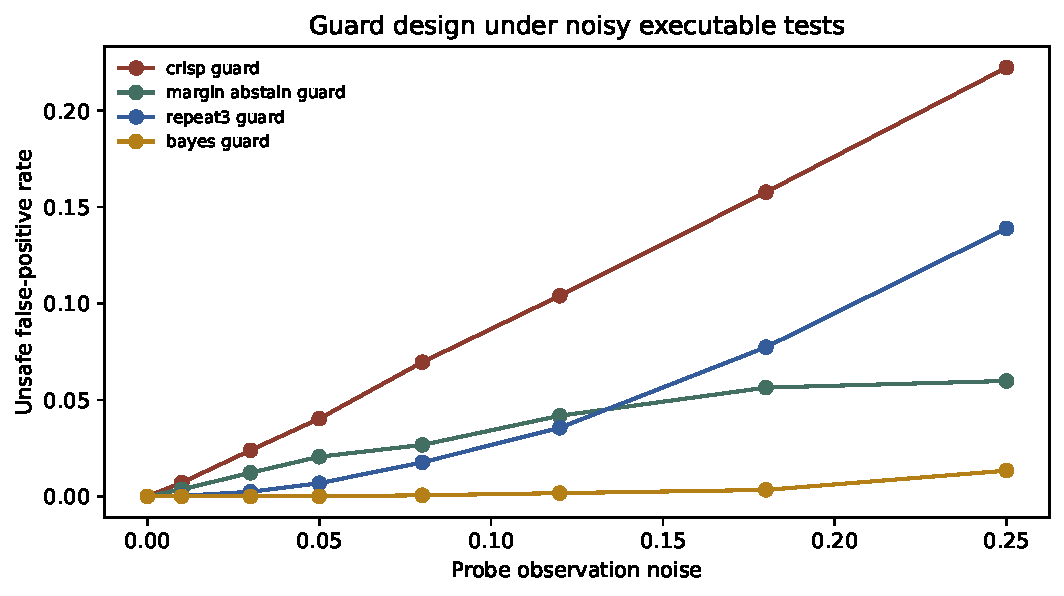
\includegraphics[width=0.82\linewidth]{../figures/full_scale/noise_guard_unsafe.pdf}
\caption{Probe-noise stress.  Repeated and abstaining guards reduce unsafe
assertions under noise, but they pay either test cost or coverage cost.}
\label{fig:noise}
\end{figure}

\begin{table}[t]
\centering
\scriptsize
\resizebox{\linewidth}{!}{\begin{tabular}{llrrrr}
\toprule
Noise & Guard & Acc. & Unsafe FP & Abstain & Test cost \\
\midrule
0.00 & bayes\_guard & 1.000 & 0.000 & 0.000 & 0.510 \\
0.00 & crisp\_guard & 1.000 & 0.000 & 0.000 & 0.102 \\
0.00 & margin\_abstain\_guard & 1.000 & 0.000 & 0.000 & 0.102 \\
0.00 & repeat3\_guard & 1.000 & 0.000 & 0.000 & 0.306 \\
0.05 & bayes\_guard & 0.979 & 0.000 & 0.021 & 0.510 \\
0.05 & crisp\_guard & 0.949 & 0.044 & 0.000 & 0.102 \\
0.05 & margin\_abstain\_guard & 0.910 & 0.018 & 0.069 & 0.102 \\
0.05 & repeat3\_guard & 0.993 & 0.006 & 0.000 & 0.306 \\
0.12 & bayes\_guard & 0.889 & 0.001 & 0.111 & 0.510 \\
0.12 & crisp\_guard & 0.875 & 0.108 & 0.000 & 0.102 \\
0.12 & margin\_abstain\_guard & 0.788 & 0.036 & 0.169 & 0.102 \\
0.12 & repeat3\_guard & 0.957 & 0.038 & 0.000 & 0.306 \\
0.25 & bayes\_guard & 0.633 & 0.014 & 0.350 & 0.510 \\
0.25 & crisp\_guard & 0.740 & 0.227 & 0.000 & 0.102 \\
0.25 & margin\_abstain\_guard & 0.580 & 0.063 & 0.349 & 0.102 \\
0.25 & repeat3\_guard & 0.839 & 0.138 & 0.000 & 0.306 \\
\bottomrule
\end{tabular}
}
\caption{Selected guard-design results under label-preserving flips.}
\label{tab:noise}
\end{table}

This family prevents a misleading reading of the positive result.  Executable
evidence is only as good as the guard and sensor model.  A deployable system
would need calibrated sensors, repeated probing when justified, and abstention
when the trace lies near the decision boundary.

\section{Passive Visibility Ladder}

The passive baseline in v2 was intentionally simple.  A reviewer could object
that a stronger vision-language model might infer holes, materials, and damage.
Family F gives passive systems progressively more visibility: label only,
geometry only, geometry plus material, geometry plus damage, a VLM-like blend of
label and visible variables, and a full noisy hidden-state proxy.  Figure
\ref{fig:visibility} and Table~\ref{tab:visibility} show that more visibility
helps substantially.  In adversarial counterfeits, label-only unsafe false
positives are 0.194, geometry-only is 0.238, geometry plus material is 0.144,
geometry plus damage is 0.141, and the VLM-like blend is 0.127.  A full noisy
hidden-state proxy reaches 0.000 unsafe false positives in this synthetic
setting.

\begin{figure}[t]
\centering
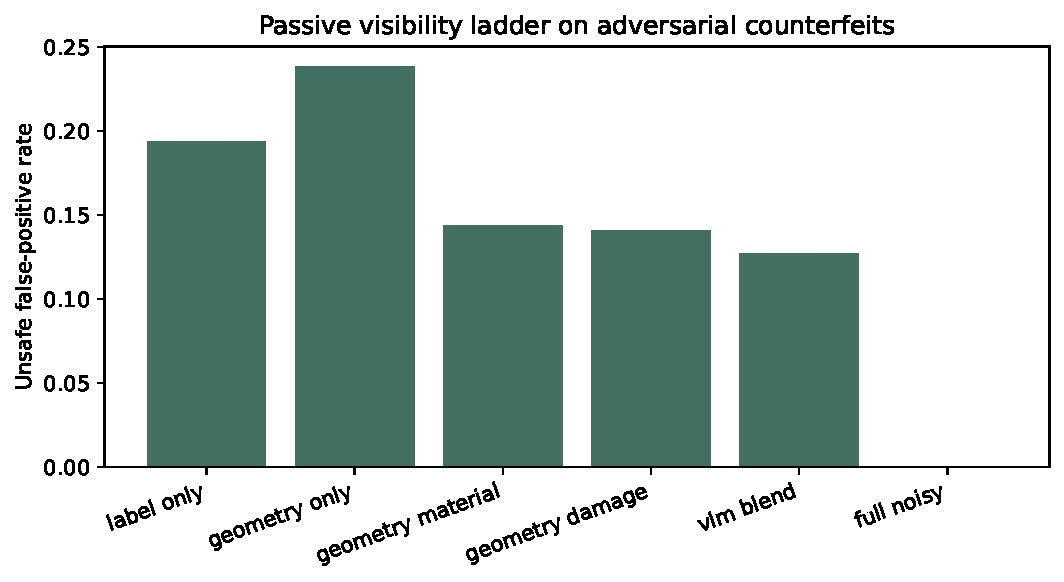
\includegraphics[width=0.82\linewidth]{../figures/full_scale/visibility_ladder.pdf}
\caption{Passive visibility ladder on adversarial counterfeits.  Better passive
visibility narrows the gap, and full observation can solve the synthetic task.
EATL is most useful when the deciding variables are hidden, stale, or
demand-specific.}
\label{fig:visibility}
\end{figure}

\begin{table}[t]
\centering
\scriptsize
\resizebox{\linewidth}{!}{\begin{tabular}{llrrrr}
\toprule
Regime & Visibility & Acc. & Unsafe FP & F1 & Total cost \\
\midrule
adversarial\_counterfeit & full\_noisy & 1.000 & 0.000 & 1.000 & 0.000 \\
adversarial\_counterfeit & geometry\_damage & 0.860 & 0.140 & 0.657 & 0.698 \\
adversarial\_counterfeit & geometry\_material & 0.857 & 0.143 & 0.651 & 0.715 \\
adversarial\_counterfeit & geometry\_only & 0.761 & 0.239 & 0.528 & 1.193 \\
adversarial\_counterfeit & label\_only & 0.804 & 0.194 & 0.572 & 0.970 \\
adversarial\_counterfeit & vlm\_blend & 0.870 & 0.129 & 0.671 & 0.645 \\
label\_preserving\_flips & full\_noisy & 1.000 & 0.000 & 1.000 & 0.000 \\
label\_preserving\_flips & geometry\_damage & 0.878 & 0.122 & 0.691 & 0.608 \\
label\_preserving\_flips & geometry\_material & 0.859 & 0.141 & 0.659 & 0.705 \\
label\_preserving\_flips & geometry\_only & 0.785 & 0.215 & 0.559 & 1.074 \\
label\_preserving\_flips & label\_only & 0.807 & 0.191 & 0.581 & 0.956 \\
label\_preserving\_flips & vlm\_blend & 0.858 & 0.142 & 0.655 & 0.709 \\
\bottomrule
\end{tabular}
}
\caption{Visibility ladder for passive systems.  The result narrows the claim:
executable tests are not needed when passive sensing already observes the
deciding physical variables reliably.}
\label{tab:visibility}
\end{table}

This is an important negative control.  EATL should not claim superiority over
a sensor that directly observes the relevant causal variables.  Its value is in
the cases where the variable is unobserved, ambiguous, stale, demand-specific,
or too consequential to trust as a category prior.

\section{Demand and Embodiment Shift}

Affordances are not object properties alone.  A container that is safe for
100ml may fail for 750ml.  A box that supports 300g may fail at 1600g.  A mug
that is safe for one robot can be unsafe for a weaker or hotter-contact
embodiment.  Family G sweeps liquid volume, load, temperature, grip force, and
robot embodiment.  The selected rows in Table~\ref{tab:demand} show the pattern:
risk-aware EATL remains low in unsafe false positives because the test is tied
to the current demand and robot, while label and passive systems often transfer
an old category-level belief across a changed physical question.

\begin{table}[t]
\centering
\scriptsize
\resizebox{\linewidth}{!}{\begin{tabular}{lllrrrr}
\toprule
Task & Value & Method & Acc. & Unsafe FP & Abstain & Total cost \\
\midrule
carry\_hot & 40 & passive\_vision\_proxy & 0.908 & 0.092 & 0.000 & 0.462 \\
carry\_hot & 40 & risk\_aware\_eatl & 0.989 & 0.005 & 0.000 & 0.058 \\
carry\_hot & 40 & text\_prior & 0.934 & 0.066 & 0.000 & 0.328 \\
carry\_hot & 60 & passive\_vision\_proxy & 0.910 & 0.090 & 0.000 & 0.451 \\
carry\_hot & 60 & risk\_aware\_eatl & 0.989 & 0.003 & 0.000 & 0.051 \\
carry\_hot & 60 & text\_prior & 0.933 & 0.067 & 0.000 & 0.337 \\
carry\_hot & 80 & passive\_vision\_proxy & 0.912 & 0.088 & 0.000 & 0.441 \\
carry\_hot & 80 & risk\_aware\_eatl & 0.991 & 0.003 & 0.000 & 0.049 \\
carry\_hot & 80 & text\_prior & 0.935 & 0.065 & 0.000 & 0.325 \\
carry\_hot & 95 & passive\_vision\_proxy & 0.725 & 0.275 & 0.000 & 1.375 \\
carry\_hot & 95 & risk\_aware\_eatl & 0.989 & 0.011 & 0.000 & 0.083 \\
carry\_hot & 95 & text\_prior & 0.750 & 0.250 & 0.000 & 1.250 \\
carry\_hot & 110 & passive\_vision\_proxy & 0.728 & 0.272 & 0.000 & 1.359 \\
carry\_hot & 110 & risk\_aware\_eatl & 0.988 & 0.012 & 0.000 & 0.090 \\
carry\_hot & 110 & text\_prior & 0.750 & 0.250 & 0.000 & 1.250 \\
carry\_hot & 130 & passive\_vision\_proxy & 0.725 & 0.275 & 0.000 & 1.373 \\
carry\_hot & 130 & risk\_aware\_eatl & 0.991 & 0.009 & 0.000 & 0.080 \\
carry\_hot & 130 & text\_prior & 0.750 & 0.250 & 0.000 & 1.250 \\
contain\_liquid & 50 & passive\_vision\_proxy & 0.821 & 0.179 & 0.000 & 0.894 \\
contain\_liquid & 50 & risk\_aware\_eatl & 0.985 & 0.007 & 0.000 & 0.084 \\
contain\_liquid & 50 & text\_prior & 0.915 & 0.082 & 0.000 & 0.412 \\
contain\_liquid & 100 & passive\_vision\_proxy & 0.826 & 0.174 & 0.000 & 0.872 \\
contain\_liquid & 100 & risk\_aware\_eatl & 0.983 & 0.007 & 0.000 & 0.086 \\
contain\_liquid & 100 & text\_prior & 0.924 & 0.071 & 0.000 & 0.357 \\
contain\_liquid & 200 & passive\_vision\_proxy & 0.820 & 0.180 & 0.000 & 0.900 \\
contain\_liquid & 200 & risk\_aware\_eatl & 0.981 & 0.009 & 0.000 & 0.098 \\
contain\_liquid & 200 & text\_prior & 0.919 & 0.076 & 0.000 & 0.385 \\
contain\_liquid & 350 & passive\_vision\_proxy & 0.900 & 0.100 & 0.000 & 0.500 \\
contain\_liquid & 350 & risk\_aware\_eatl & 0.987 & 0.008 & 0.000 & 0.083 \\
contain\_liquid & 350 & text\_prior & 0.831 & 0.166 & 0.000 & 0.834 \\
contain\_liquid & 500 & passive\_vision\_proxy & 0.948 & 0.052 & 0.000 & 0.259 \\
contain\_liquid & 500 & risk\_aware\_eatl & 0.988 & 0.008 & 0.000 & 0.083 \\
contain\_liquid & 500 & text\_prior & 0.790 & 0.207 & 0.000 & 1.036 \\
contain\_liquid & 750 & passive\_vision\_proxy & 0.965 & 0.035 & 0.000 & 0.174 \\
contain\_liquid & 750 & risk\_aware\_eatl & 0.985 & 0.015 & 0.000 & 0.116 \\
contain\_liquid & 750 & text\_prior & 0.699 & 0.298 & 0.000 & 1.492 \\
grasp\_without\_crushing & 4 & passive\_vision\_proxy & 0.831 & 0.169 & 0.000 & 0.844 \\
grasp\_without\_crushing & 4 & risk\_aware\_eatl & 0.967 & 0.008 & 0.000 & 0.147 \\
grasp\_without\_crushing & 4 & text\_prior & 0.678 & 0.083 & 0.000 & 0.558 \\
grasp\_without\_crushing & 8 & passive\_vision\_proxy & 0.747 & 0.253 & 0.000 & 1.267 \\
grasp\_without\_crushing & 8 & risk\_aware\_eatl & 0.970 & 0.012 & 0.000 & 0.163 \\
grasp\_without\_crushing & 8 & text\_prior & 0.761 & 0.088 & 0.000 & 0.530 \\
grasp\_without\_crushing & 14 & passive\_vision\_proxy & 0.598 & 0.402 & 0.000 & 2.012 \\
grasp\_without\_crushing & 14 & risk\_aware\_eatl & 0.964 & 0.017 & 0.000 & 0.189 \\
grasp\_without\_crushing & 14 & text\_prior & 0.869 & 0.107 & 0.000 & 0.549 \\
grasp\_without\_crushing & 20 & passive\_vision\_proxy & 0.525 & 0.475 & 0.000 & 2.377 \\
grasp\_without\_crushing & 20 & risk\_aware\_eatl & 0.967 & 0.021 & 0.000 & 0.205 \\
grasp\_without\_crushing & 20 & text\_prior & 0.845 & 0.155 & 0.000 & 0.774 \\
grasp\_without\_crushing & 30 & passive\_vision\_proxy & 0.413 & 0.587 & 0.000 & 2.933 \\
grasp\_without\_crushing & 30 & risk\_aware\_eatl & 0.972 & 0.020 & 0.000 & 0.203 \\
grasp\_without\_crushing & 30 & text\_prior & 0.736 & 0.264 & 0.000 & 1.321 \\
grasp\_without\_crushing & 45 & passive\_vision\_proxy & 0.285 & 0.715 & 0.000 & 3.573 \\
grasp\_without\_crushing & 45 & risk\_aware\_eatl & 0.972 & 0.023 & 0.000 & 0.225 \\
grasp\_without\_crushing & 45 & text\_prior & 0.615 & 0.385 & 0.000 & 1.927 \\
\bottomrule
\end{tabular}
}
\caption{Selected demand and embodiment shift rows.  The same object label can
change truth value as volume, load, temperature, grip force, or robot body
changes.}
\label{tab:demand}
\end{table}

The lesson is not that demand sweeps are exotic.  They are the normal form of a
robot affordance claim.  A predicate such as \texttt{can-support-load} is
incomplete until the load and robot are specified.  A cached witness that omits
the demand is not a full witness.

\section{Failure Gallery}

The failure gallery in Table~\ref{tab:gallery} is not meant as qualitative
hardware evidence.  It is a compact audit trail.  The examples show unsafe
false positives, avoidable false negatives, abstentions, saved tests, and
irrelevant-test failures.  They make the synthetic mechanism inspectable: a row
contains the object, task, method, decision, witness text, demand, robot, and
hidden state.  This is useful for reviewers because it exposes exactly what the
benchmark is and is not testing.

\begin{table}[t]
\centering
\scriptsize
\resizebox{\linewidth}{!}{\begin{tabular}{lllllp{0.35\linewidth}}
\toprule
Kind & Regime & Object & Task & Method & Witness \\
\midrule
abstention & typical & mug & contain\_liquid & conservative\_prior & conservative\_prior(abstain) \\
saved\_test\_correct & typical & mug & support\_load & risk\_aware\_eatl & risk\_aware\_eatl(reject,p=0.06) \\
saved\_test\_correct & typical & mug & wipe\_spill & risk\_aware\_eatl & risk\_aware\_eatl(reject,p=0.06) \\
unsafe\_false\_positive & typical & mug & wipe\_spill & random\_test\_control & irrelevant\_random\_probe \\
abstention & typical & mug & carry\_hot & conservative\_prior & conservative\_prior(abstain) \\
avoidable\_false\_negative & typical & mug & carry\_hot & random\_test\_control & irrelevant\_random\_probe \\
abstention & typical & mug & pour\_without\_spill & conservative\_prior & conservative\_prior(abstain) \\
saved\_test\_correct & typical & mug & stack\_safely & risk\_aware\_eatl & risk\_aware\_eatl(reject,p=0.16) \\
abstention & typical & mug & grasp\_without\_crushing & conservative\_prior & conservative\_prior(abstain) \\
avoidable\_false\_negative & typical & mug & grasp\_without\_crushing & random\_test\_control & irrelevant\_random\_probe \\
abstention & typical & bowl & contain\_liquid & conservative\_prior & conservative\_prior(abstain) \\
avoidable\_false\_negative & typical & bowl & contain\_liquid & random\_test\_control & irrelevant\_random\_probe \\
unsafe\_false\_positive & typical & bowl & support\_load & random\_test\_control & irrelevant\_random\_probe \\
saved\_test\_correct & typical & bowl & cut\_soft\_food & risk\_aware\_eatl & risk\_aware\_eatl(reject,p=0.16) \\
saved\_test\_correct & typical & bowl & wipe\_spill & risk\_aware\_eatl & risk\_aware\_eatl(reject,p=0.06) \\
unsafe\_false\_positive & typical & bowl & wipe\_spill & random\_test\_control & irrelevant\_random\_probe \\
saved\_test\_correct & typical & bowl & carry\_hot & risk\_aware\_eatl & risk\_aware\_eatl(reject,p=0.15) \\
saved\_test\_correct & typical & bowl & pour\_without\_spill & risk\_aware\_eatl & risk\_aware\_eatl(reject,p=0.16) \\
\bottomrule
\end{tabular}
}
\caption{Representative failure-gallery rows.  The full CSV records bounded
examples from the main family.}
\label{tab:gallery}
\end{table}

\section{Discussion}

The main conceptual shift is from facts to evidence.  A text prior says a mug
usually contains liquid.  An EATL witness says this object, with this robot, for
this demanded volume, passed a diagnostic relation that licenses the predicate.
The difference matters because many robot errors are not caused by ignorance of
ordinary object categories; they are caused by ordinary categories hiding
changed physics.

The second shift is from confidence to certificate.  A failed test is not merely
a lower probability.  It is a local reason the planner can use: this container
leaks, this support cannot carry the demanded load, this edge is too dull, this
grasp would crush the object.  Such certificates can support recovery, object
substitution, user queries, or cache invalidation.

The third shift is that testing must be selected.  The phase diagram shows
regions where text or conservative priors are cheaper.  The cache experiment
shows that reuse can be beneficial.  The visibility ladder shows that passive
sensing can close the gap when it sees the deciding variable.  The noise sweep
shows that tests require robust guards.  These are not problems for the
semantics; they are requirements for implementing it honestly.

\section{Limitations}

The most important limitation is that the evidence is synthetic.  There is no
real robot, no tactile sensor, no photorealistic simulator, and no learned test
program.  The environment is a transparent mechanism test, not a deployment
benchmark.  The paper should be read as evidence that a field assumption is
dangerous, not as evidence that a particular robot system is ready.

The second limitation is that the tests are hand-specified.  In practice,
micro-policies and guards would need to be learned, synthesized, verified, or
calibrated for the robot and sensor suite.  Some tests are destructive or
expensive.  A thermal test, load test, or crushing test can change the object.
The phase diagram and noise experiments make this limitation explicit, but they
do not solve it.

The third limitation is that the cost model is simplified.  False positives,
false negatives, test costs, abstentions, and sensor errors are represented by
normalized synthetic costs.  Real deployments need task-specific harm models,
human preferences, legal constraints, and repair costs.

The fourth limitation is that the formal results are simple.  The label-only
bound does not apply to all multimodal systems.  A passive system that observes
all relevant hidden variables can solve the synthetic task, as the visibility
ladder confirms.  The novelty claim is therefore not that EATL beats every
model, but that embodied common-sense assertions should be tied to executable
evidence and validity conditions.

\section{Conclusion}

Robots fail when familiar words hide changed physics.  We proposed Executable
Affordance Test Logic, a semantics in which robotic common-sense predicates are
licensed by executable witnesses rather than object names alone.  The v3
full-scale synthetic evaluation shows that risk-aware executable witnesses
reduce unsafe false positives under hidden same-name changes, adversarial
counterfeits, demand shifts, and embodiment shifts.  It also shows the
boundary: when probes are expensive, hidden flips are rare, caches are stale, or
passive sensing observes the deciding variables, testing can be unnecessary or
unsafe.  The next step is to learn or synthesize executable tests and evaluate
them on real robot manipulation tasks with measured test costs, calibrated
guards, and explicit witness validity.

\subsubsection*{Reproducibility Statement}
The v3 full-scale evidence is reproduced with:
\begin{verbatim}
python experiments/full_scale_affordance_tests.py
python scripts/render_full_scale_figures.py
powershell -ExecutionPolicy Bypass -File scripts/build_pdf.ps1
\end{verbatim}
The runner writes aggregate CSVs to \texttt{results/full\_scale/}, LaTeX tables
to \texttt{paper/}, and figures to \texttt{figures/full\_scale/}.  The v3 run
completed in 437.075 seconds, used deterministic seed families 28001--28612,
and retained aggregate counters rather than full raw logs.  The older v2
experiment remains reproducible with \texttt{python experiments/affordance\_tests.py}
and \texttt{python scripts/write\_paper\_assets.py}.

\bibliography{references}
\bibliographystyle{iclr2026_conference}

\appendix

\section{Appendix A: Predicate Semantics}

This appendix expands the semantics used in the main text.  The point is to
avoid a common ambiguity: an affordance can be a possible action, a perceived
cue, a predicted success probability, a symbolic precondition, or a planner
feasibility check.  EATL uses the word in a narrower operational sense.  A robot
may assert an affordance predicate only when it has an executable witness whose
validity scope covers the current tuple.

\paragraph{Pass, fail, and abstain.}
A pass trace is evidence for an assertion.  A fail trace is a certificate
against assertion.  An abstain trace is a refusal to license either direction.
Abstention is needed because some tests are too noisy, too expensive, or too
dangerous.  In the synthetic experiments, abstention appears most clearly in
the conservative prior and margin or Bayesian guards.  In a real system,
abstention would trigger escalation: ask a human, choose a safer object, select
a different skill, or run a more expensive test.

\paragraph{Validity scope.}
A witness is scoped by object state, robot embodiment, task demand, and time.
If a mug passes a 200ml containment test, the witness does not automatically
license a 750ml pour.  If a gripper changes, a lift witness may expire.  If a
box gets wet, a support-load witness may expire.  The cache experiment is built
around this rule.  Strict validity reuse saves cost; label-only reuse collapses
back into the mistake EATL was meant to avoid.

\paragraph{Failure certificates.}
Failure certificates are useful because they are local.  A failed
\texttt{can-contain-liquid} witness does not imply that the object cannot be
lifted or stacked.  It says the object did not satisfy a particular predicate
under a particular demand.  This local structure lets a planner replace only the
failed relation rather than discarding a whole plan.

\section{Appendix B: Environment Details}

Each object instance is represented by a small vector of physical variables.
The variables are not intended to be complete physics; they are chosen to make
the benchmark inspectable.  The hidden variables include:

\begin{itemize}
\item containment variables: concavity, porosity, holes, capacity, pour lip,
and stability;
\item manipulation variables: mass, friction, grippability, crush limit, and
surface fragility;
\item tool variables: sharpness, edge stiffness, absorbency, heat resistance,
and handle availability;
\item support variables: load capacity, flat top, stable base, wetness, and
degradation.
\end{itemize}

Ground-truth predicates are deterministic threshold functions.  For example,
containment requires concavity, no hole, non-porosity, capacity above demanded
volume, and a stable base.  Support requires load capacity above the demanded
load, a stable base, and a flat top.  Grasp-without-crushing requires that the
object be grippable, within the robot's gripper limit, below the surface
fragility threshold, and above the demanded crush-force margin.

\paragraph{Why deterministic truth is acceptable here.}
The paper is not estimating real-world success probabilities.  It is isolating
a representation failure: labels can remain fixed while causal variables
change.  Deterministic truth makes the failure mode inspectable.  Noise is then
introduced in the test observations and guard policies rather than hidden
inside the ground-truth simulator.

\paragraph{Regime construction.}
The label-preserving flip regime samples hidden mutations such as adding a hole,
making an object porous, dulling an edge, increasing mass, reducing load
capacity, removing heat resistance, eliminating absorbency, removing a pour lip,
lowering crush limit, or destabilizing the base.  The adversarial counterfeit
regime chooses mutations that specifically target a predicate that the label
prior believes is true.  The task-demand regime changes the question rather
than the object.  The embodiment regime changes robot limits.

\section{Appendix C: Method Details}

\paragraph{Text prior.}
The text prior is derived from the typical object catalog.  If the typical mug
contains liquid, the prior asserts containment for all mugs.  This makes it
strong on typical objects and vulnerable under same-name hidden changes.

\paragraph{Calibrated text prior.}
The calibrated text prior weakens confidence in hostile regimes.  It can abstain
near its boundary.  This baseline addresses the objection that no reasonable
system would use an uncalibrated label prior in a known hostile setting.

\paragraph{Passive and uncertainty-aware vision proxies.}
The passive proxy observes geometry-like variables: concavity, flatness,
stability, and approximate mass.  It misses hidden material, holes, damage, and
demand-specific safety margins.  The uncertainty-aware version also abstains
when its score lies near the boundary.  Family F gives passive systems more
visibility to show where EATL is and is not needed.

\paragraph{Conservative prior.}
The conservative prior asserts only high-confidence, low-consequence positive
predicates, rejects confident negatives, and abstains otherwise.  It is a strong
safety baseline because it can reduce unsafe false positives by refusing to act.
Its weakness is coverage and avoidable false negatives.

\paragraph{Eager EATL.}
Eager EATL always runs the task-specific test and uses the noisy test result.
It is useful as a mechanism upper baseline, but it can be dominated when hidden
flips are rare or tests are costly.

\paragraph{Risk-aware EATL.}
Risk-aware EATL blends label and visible evidence, estimates the expected harm
of assertion or rejection, compares the value of testing to test cost, and runs
the test only when it appears worthwhile.  It is not globally optimal; it is a
simple selector designed to expose the difference between executable evidence
and eager evidence gathering.

\paragraph{Cached EATL.}
Cached EATL stores strict witnesses keyed by current state, task demand, and
robot embodiment.  The separate cache family compares this strict reuse against
label-only, time-to-live, and demand-compatible reuse.

\section{Appendix D: Additional Tables}

\subsection{D.1 Main Task-Level Outputs}

The repository contains \texttt{results/full\_scale/main\_task\_summary.csv}
with per-task, per-regime, per-method aggregates.  Those rows are not all
included in the PDF because they are too large for readable page layout, but
they are used to audit whether the main effects come from one predicate.  The
pattern is broad: label priors fail most sharply for containment, hot carrying,
pouring, and crushing, while passive geometry has particular trouble with
material and damage variables.

\subsection{D.2 Demand and Embodiment Table}

Table~\ref{tab:demand} in the main text shows selected demand and embodiment
rows.  The full CSV includes 648 seed-summary rows and 129,600 method decisions.
The most useful interpretation is that demand is part of the predicate.  A
single object label cannot define a support-load, containment, or thermal
affordance without the demanded quantity.

\subsection{D.3 Failure Gallery}

The failure gallery CSV stores bounded representative examples rather than full
raw logs.  This keeps memory and repository size under control while preserving
inspectability.  A reviewer can trace a reported false positive to an object
state and witness string.

\section{Appendix E: Full Experiment Accounting}

The aggregate decision counts are:

\begin{center}
\begin{tabular}{lrr}
\toprule
Family & Seed-summary rows & Method decisions \\
\midrule
Main benchmark & 960 & 1,920,000 \\
Phase diagram & 3,360 & 2,016,000 \\
Selector ablation & 168 & 268,800 \\
Cache validity & 40 & 240,000 \\
Noise and guard design & 192 & 230,400 \\
Visibility ladder & 108 & 172,800 \\
Demand and embodiment & 648 & 129,600 \\
\midrule
Total & 5,476 & 4,977,600 \\
\bottomrule
\end{tabular}
\end{center}

The runner uses deterministic seeds and writes seed-level summaries before
aggregate summaries.  Means and standard errors are computed across seeds.  Raw
case rows are not retained for the full benchmark because they would be large
and unnecessary for the reported metrics.  Instead, bounded representative
examples are written to the failure gallery.

\section{Appendix F: Complete V3 Result Tables}

The main text includes compact tables for readability.  This appendix includes
larger result grids generated directly from the v3 CSV outputs.  They are not
additional claims; they are audit material for checking whether a result is
concentrated in one regime, task, or cost setting.

\subsection{F.1 Full Main Benchmark}

\begingroup
\scriptsize
\begin{longtable}{llrrrrrr}
\toprule
Regime & Method & Acc. & Unsafe FP & FN & Abstain & Test & Total \\
\midrule
\endfirsthead
\toprule
Regime & Method & Acc. & Unsafe FP & FN & Abstain & Test & Total \\
\midrule
\endhead
typical & text prior & 0.994 & 0.004 & 0.002 & 0.000 & 0.000 & 0.024 \\
typical & calibrated text prior & 0.994 & 0.004 & 0.002 & 0.000 & 0.000 & 0.024 \\
typical & passive vision proxy & 0.823 & 0.177 & 0.000 & 0.000 & 0.000 & 0.883 \\
typical & uncertainty vision proxy & 0.823 & 0.090 & 0.000 & 0.087 & 0.000 & 0.463 \\
typical & conservative prior & 0.849 & 0.004 & 0.002 & 0.145 & 0.000 & 0.045 \\
typical & eager eatl & 0.975 & 0.016 & 0.009 & 0.000 & 0.102 & 0.189 \\
typical & risk aware eatl & 0.987 & 0.005 & 0.008 & 0.000 & 0.055 & 0.087 \\
typical & cached eatl & 0.974 & 0.017 & 0.009 & 0.000 & 0.102 & 0.193 \\
typical & oracle hidden state & 1.000 & 0.000 & 0.000 & 0.000 & 0.000 & 0.000 \\
typical & random test control & 0.499 & 0.338 & 0.163 & 0.000 & 0.066 & 1.853 \\
\midrule
label preserving flips & text prior & 0.810 & 0.188 & 0.002 & 0.000 & 0.000 & 0.940 \\
label preserving flips & calibrated text prior & 0.810 & 0.188 & 0.002 & 0.000 & 0.000 & 0.940 \\
label preserving flips & passive vision proxy & 0.788 & 0.212 & 0.000 & 0.000 & 0.000 & 1.059 \\
label preserving flips & uncertainty vision proxy & 0.788 & 0.100 & 0.000 & 0.111 & 0.000 & 0.519 \\
label preserving flips & conservative prior & 0.739 & 0.113 & 0.002 & 0.145 & 0.000 & 0.590 \\
label preserving flips & eager eatl & 0.975 & 0.022 & 0.004 & 0.000 & 0.102 & 0.213 \\
label preserving flips & risk aware eatl & 0.981 & 0.015 & 0.004 & 0.000 & 0.070 & 0.150 \\
label preserving flips & cached eatl & 0.974 & 0.022 & 0.004 & 0.000 & 0.101 & 0.216 \\
label preserving flips & oracle hidden state & 1.000 & 0.000 & 0.000 & 0.000 & 0.000 & 0.000 \\
label preserving flips & random test control & 0.498 & 0.429 & 0.072 & 0.000 & 0.066 & 2.256 \\
\midrule
label swap & text prior & 0.669 & 0.166 & 0.165 & 0.000 & 0.000 & 0.929 \\
label swap & calibrated text prior & 0.669 & 0.166 & 0.165 & 0.000 & 0.000 & 0.929 \\
label swap & passive vision proxy & 0.826 & 0.174 & 0.000 & 0.000 & 0.000 & 0.873 \\
label swap & uncertainty vision proxy & 0.826 & 0.089 & 0.000 & 0.086 & 0.000 & 0.456 \\
label swap & conservative prior & 0.618 & 0.073 & 0.165 & 0.145 & 0.000 & 0.484 \\
label swap & eager eatl & 0.973 & 0.018 & 0.009 & 0.000 & 0.102 & 0.196 \\
label swap & risk aware eatl & 0.985 & 0.008 & 0.008 & 0.000 & 0.065 & 0.107 \\
label swap & cached eatl & 0.974 & 0.017 & 0.009 & 0.000 & 0.082 & 0.173 \\
label swap & oracle hidden state & 1.000 & 0.000 & 0.000 & 0.000 & 0.000 & 0.000 \\
label swap & random test control & 0.496 & 0.340 & 0.164 & 0.000 & 0.066 & 1.864 \\
\midrule
mixed & text prior & 0.821 & 0.121 & 0.058 & 0.000 & 0.000 & 0.639 \\
mixed & calibrated text prior & 0.821 & 0.121 & 0.058 & 0.000 & 0.000 & 0.639 \\
mixed & passive vision proxy & 0.810 & 0.190 & 0.000 & 0.000 & 0.000 & 0.952 \\
mixed & uncertainty vision proxy & 0.810 & 0.093 & 0.000 & 0.097 & 0.000 & 0.480 \\
mixed & conservative prior & 0.732 & 0.065 & 0.058 & 0.145 & 0.000 & 0.381 \\
mixed & eager eatl & 0.974 & 0.019 & 0.007 & 0.000 & 0.102 & 0.202 \\
mixed & risk aware eatl & 0.984 & 0.009 & 0.007 & 0.000 & 0.058 & 0.109 \\
mixed & cached eatl & 0.973 & 0.020 & 0.007 & 0.000 & 0.086 & 0.191 \\
mixed & oracle hidden state & 1.000 & 0.000 & 0.000 & 0.000 & 0.000 & 0.000 \\
mixed & random test control & 0.497 & 0.372 & 0.132 & 0.000 & 0.066 & 2.004 \\
\midrule
adversarial counterfeit & text prior & 0.800 & 0.197 & 0.002 & 0.000 & 0.000 & 0.988 \\
adversarial counterfeit & calibrated text prior & 0.800 & 0.197 & 0.002 & 0.000 & 0.000 & 0.988 \\
adversarial counterfeit & passive vision proxy & 0.760 & 0.240 & 0.000 & 0.000 & 0.000 & 1.201 \\
adversarial counterfeit & uncertainty vision proxy & 0.760 & 0.107 & 0.000 & 0.133 & 0.000 & 0.554 \\
adversarial counterfeit & conservative prior & 0.739 & 0.114 & 0.002 & 0.145 & 0.000 & 0.594 \\
adversarial counterfeit & eager eatl & 0.958 & 0.037 & 0.006 & 0.000 & 0.102 & 0.288 \\
adversarial counterfeit & risk aware eatl & 0.970 & 0.025 & 0.005 & 0.000 & 0.078 & 0.205 \\
adversarial counterfeit & cached eatl & 0.957 & 0.038 & 0.005 & 0.000 & 0.088 & 0.281 \\
adversarial counterfeit & oracle hidden state & 1.000 & 0.000 & 0.000 & 0.000 & 0.000 & 0.000 \\
adversarial counterfeit & random test control & 0.505 & 0.431 & 0.064 & 0.000 & 0.066 & 2.260 \\
\midrule
degraded worn & text prior & 0.849 & 0.151 & 0.000 & 0.000 & 0.000 & 0.757 \\
degraded worn & calibrated text prior & 0.849 & 0.151 & 0.000 & 0.000 & 0.000 & 0.757 \\
degraded worn & passive vision proxy & 0.758 & 0.242 & 0.000 & 0.000 & 0.000 & 1.209 \\
degraded worn & uncertainty vision proxy & 0.758 & 0.092 & 0.000 & 0.150 & 0.000 & 0.482 \\
degraded worn & conservative prior & 0.752 & 0.103 & 0.000 & 0.145 & 0.000 & 0.535 \\
degraded worn & eager eatl & 0.957 & 0.035 & 0.007 & 0.000 & 0.102 & 0.282 \\
degraded worn & risk aware eatl & 0.971 & 0.021 & 0.007 & 0.000 & 0.071 & 0.183 \\
degraded worn & cached eatl & 0.960 & 0.034 & 0.007 & 0.000 & 0.102 & 0.274 \\
degraded worn & oracle hidden state & 1.000 & 0.000 & 0.000 & 0.000 & 0.000 & 0.000 \\
degraded worn & random test control & 0.497 & 0.415 & 0.087 & 0.000 & 0.066 & 2.195 \\
\midrule
task demand shift & text prior & 0.922 & 0.057 & 0.021 & 0.000 & 0.000 & 0.296 \\
task demand shift & calibrated text prior & 0.922 & 0.057 & 0.021 & 0.000 & 0.000 & 0.296 \\
task demand shift & passive vision proxy & 0.814 & 0.186 & 0.000 & 0.000 & 0.000 & 0.931 \\
task demand shift & uncertainty vision proxy & 0.814 & 0.106 & 0.000 & 0.080 & 0.000 & 0.542 \\
task demand shift & conservative prior & 0.816 & 0.018 & 0.021 & 0.145 & 0.000 & 0.123 \\
task demand shift & eager eatl & 0.973 & 0.019 & 0.008 & 0.000 & 0.106 & 0.206 \\
task demand shift & risk aware eatl & 0.985 & 0.007 & 0.008 & 0.000 & 0.057 & 0.097 \\
task demand shift & cached eatl & 0.974 & 0.019 & 0.007 & 0.000 & 0.106 & 0.205 \\
task demand shift & oracle hidden state & 1.000 & 0.000 & 0.000 & 0.000 & 0.000 & 0.000 \\
task demand shift & random test control & 0.500 & 0.353 & 0.147 & 0.000 & 0.069 & 1.924 \\
\midrule
embodiment shift & text prior & 0.963 & 0.035 & 0.003 & 0.000 & 0.000 & 0.175 \\
embodiment shift & calibrated text prior & 0.963 & 0.035 & 0.003 & 0.000 & 0.000 & 0.175 \\
embodiment shift & passive vision proxy & 0.801 & 0.199 & 0.000 & 0.000 & 0.000 & 0.995 \\
embodiment shift & uncertainty vision proxy & 0.801 & 0.106 & 0.000 & 0.093 & 0.000 & 0.545 \\
embodiment shift & conservative prior & 0.838 & 0.015 & 0.003 & 0.145 & 0.000 & 0.098 \\
embodiment shift & eager eatl & 0.952 & 0.034 & 0.014 & 0.000 & 0.102 & 0.280 \\
embodiment shift & risk aware eatl & 0.975 & 0.012 & 0.013 & 0.000 & 0.056 & 0.124 \\
embodiment shift & cached eatl & 0.955 & 0.032 & 0.013 & 0.000 & 0.102 & 0.270 \\
embodiment shift & oracle hidden state & 1.000 & 0.000 & 0.000 & 0.000 & 0.000 & 0.000 \\
embodiment shift & random test control & 0.497 & 0.356 & 0.147 & 0.000 & 0.066 & 1.936 \\
\bottomrule
\end{longtable}

\endgroup

\subsection{F.2 Task-Level Breakdown}

The task-level table covers four hostile or shifting regimes and six main
methods.  It is useful for seeing which predicates drive the main effect.  The
unsafe assertion failures are broad rather than confined to one predicate:
containment, pouring, hot carrying, support, and crushing all expose cases where
labels and passive geometry are insufficient.

\begingroup
\tiny
\begin{longtable}{lllrrrrr}
\toprule
Regime & Task & Method & Acc. & Unsafe FP & Abstain & Test & Total \\
\midrule
\endfirsthead
\toprule
Regime & Task & Method & Acc. & Unsafe FP & Abstain & Test & Total \\
\midrule
\endhead
adversarial counterfeit & carry hot & cached eatl & 0.959 & 0.037 & 0.000 & 0.086 & 0.274 \\
adversarial counterfeit & carry hot & conservative prior & 0.750 & 0.000 & 0.250 & 0.000 & 0.038 \\
adversarial counterfeit & carry hot & eager eatl & 0.950 & 0.039 & 0.000 & 0.100 & 0.302 \\
adversarial counterfeit & carry hot & passive vision proxy & 0.892 & 0.108 & 0.000 & 0.000 & 0.540 \\
adversarial counterfeit & carry hot & risk aware eatl & 0.972 & 0.019 & 0.000 & 0.060 & 0.159 \\
adversarial counterfeit & carry hot & text prior & 0.887 & 0.113 & 0.000 & 0.000 & 0.562 \\
\midrule
adversarial counterfeit & contain liquid & cached eatl & 0.948 & 0.045 & 0.000 & 0.086 & 0.317 \\
adversarial counterfeit & contain liquid & conservative prior & 0.693 & 0.000 & 0.300 & 0.000 & 0.049 \\
adversarial counterfeit & contain liquid & eager eatl & 0.963 & 0.030 & 0.000 & 0.100 & 0.252 \\
adversarial counterfeit & contain liquid & passive vision proxy & 0.746 & 0.254 & 0.000 & 0.000 & 1.271 \\
adversarial counterfeit & contain liquid & risk aware eatl & 0.964 & 0.028 & 0.000 & 0.082 & 0.225 \\
adversarial counterfeit & contain liquid & text prior & 0.859 & 0.135 & 0.000 & 0.000 & 0.677 \\
\midrule
adversarial counterfeit & cut soft food & cached eatl & 0.963 & 0.037 & 0.000 & 0.104 & 0.291 \\
adversarial counterfeit & cut soft food & conservative prior & 0.988 & 0.012 & 0.000 & 0.000 & 0.060 \\
adversarial counterfeit & cut soft food & eager eatl & 0.961 & 0.037 & 0.000 & 0.120 & 0.305 \\
adversarial counterfeit & cut soft food & passive vision proxy & 0.650 & 0.350 & 0.000 & 0.000 & 1.750 \\
adversarial counterfeit & cut soft food & risk aware eatl & 0.960 & 0.037 & 0.000 & 0.120 & 0.309 \\
adversarial counterfeit & cut soft food & text prior & 0.988 & 0.012 & 0.000 & 0.000 & 0.060 \\
\midrule
adversarial counterfeit & grasp without crushing & cached eatl & 0.950 & 0.039 & 0.000 & 0.086 & 0.289 \\
adversarial counterfeit & grasp without crushing & conservative prior & 0.450 & 0.000 & 0.550 & 0.000 & 0.083 \\
adversarial counterfeit & grasp without crushing & eager eatl & 0.960 & 0.035 & 0.000 & 0.100 & 0.280 \\
adversarial counterfeit & grasp without crushing & passive vision proxy & 0.609 & 0.391 & 0.000 & 0.000 & 1.954 \\
adversarial counterfeit & grasp without crushing & risk aware eatl & 0.965 & 0.030 & 0.000 & 0.100 & 0.251 \\
adversarial counterfeit & grasp without crushing & text prior & 0.647 & 0.353 & 0.000 & 0.000 & 1.765 \\
\midrule
adversarial counterfeit & lift & cached eatl & 0.953 & 0.035 & 0.000 & 0.069 & 0.251 \\
adversarial counterfeit & lift & conservative prior & 0.482 & 0.507 & 0.000 & 0.000 & 2.540 \\
adversarial counterfeit & lift & eager eatl & 0.959 & 0.025 & 0.000 & 0.080 & 0.216 \\
adversarial counterfeit & lift & passive vision proxy & 0.767 & 0.233 & 0.000 & 0.000 & 1.167 \\
adversarial counterfeit & lift & risk aware eatl & 0.963 & 0.027 & 0.000 & 0.080 & 0.221 \\
adversarial counterfeit & lift & text prior & 0.482 & 0.507 & 0.000 & 0.000 & 2.540 \\
\midrule
adversarial counterfeit & pour without spill & cached eatl & 0.955 & 0.041 & 0.000 & 0.104 & 0.311 \\
adversarial counterfeit & pour without spill & conservative prior & 0.800 & 0.000 & 0.200 & 0.000 & 0.030 \\
adversarial counterfeit & pour without spill & eager eatl & 0.954 & 0.044 & 0.000 & 0.120 & 0.342 \\
adversarial counterfeit & pour without spill & passive vision proxy & 0.762 & 0.237 & 0.000 & 0.000 & 1.188 \\
adversarial counterfeit & pour without spill & risk aware eatl & 0.971 & 0.027 & 0.000 & 0.089 & 0.226 \\
adversarial counterfeit & pour without spill & text prior & 0.857 & 0.143 & 0.000 & 0.000 & 0.715 \\
\midrule
adversarial counterfeit & push without sliding & cached eatl & 0.962 & 0.030 & 0.000 & 0.078 & 0.235 \\
adversarial counterfeit & push without sliding & conservative prior & 0.619 & 0.376 & 0.000 & 0.000 & 1.884 \\
adversarial counterfeit & push without sliding & eager eatl & 0.960 & 0.034 & 0.000 & 0.090 & 0.263 \\
adversarial counterfeit & push without sliding & passive vision proxy & 0.950 & 0.050 & 0.000 & 0.000 & 0.250 \\
adversarial counterfeit & push without sliding & risk aware eatl & 0.965 & 0.027 & 0.000 & 0.090 & 0.229 \\
adversarial counterfeit & push without sliding & text prior & 0.619 & 0.376 & 0.000 & 0.000 & 1.884 \\
\midrule
adversarial counterfeit & stack safely & cached eatl & 0.959 & 0.039 & 0.000 & 0.095 & 0.292 \\
adversarial counterfeit & stack safely & conservative prior & 0.853 & 0.147 & 0.000 & 0.000 & 0.735 \\
adversarial counterfeit & stack safely & eager eatl & 0.953 & 0.046 & 0.000 & 0.110 & 0.340 \\
adversarial counterfeit & stack safely & passive vision proxy & 0.797 & 0.203 & 0.000 & 0.000 & 1.012 \\
adversarial counterfeit & stack safely & risk aware eatl & 0.974 & 0.024 & 0.000 & 0.066 & 0.186 \\
adversarial counterfeit & stack safely & text prior & 0.853 & 0.147 & 0.000 & 0.000 & 0.735 \\
\midrule
adversarial counterfeit & support load & cached eatl & 0.961 & 0.037 & 0.000 & 0.112 & 0.301 \\
adversarial counterfeit & support load & conservative prior & 0.850 & 0.000 & 0.150 & 0.000 & 0.022 \\
adversarial counterfeit & support load & eager eatl & 0.962 & 0.035 & 0.000 & 0.130 & 0.308 \\
adversarial counterfeit & support load & passive vision proxy & 0.805 & 0.195 & 0.000 & 0.000 & 0.973 \\
adversarial counterfeit & support load & risk aware eatl & 0.981 & 0.015 & 0.000 & 0.058 & 0.135 \\
adversarial counterfeit & support load & text prior & 0.911 & 0.089 & 0.000 & 0.000 & 0.446 \\
\midrule
adversarial counterfeit & wipe spill & cached eatl & 0.962 & 0.037 & 0.000 & 0.061 & 0.248 \\
adversarial counterfeit & wipe spill & conservative prior & 0.900 & 0.100 & 0.000 & 0.000 & 0.498 \\
adversarial counterfeit & wipe spill & eager eatl & 0.957 & 0.040 & 0.000 & 0.070 & 0.272 \\
adversarial counterfeit & wipe spill & passive vision proxy & 0.619 & 0.381 & 0.000 & 0.000 & 1.904 \\
adversarial counterfeit & wipe spill & risk aware eatl & 0.984 & 0.015 & 0.000 & 0.034 & 0.109 \\
adversarial counterfeit & wipe spill & text prior & 0.900 & 0.100 & 0.000 & 0.000 & 0.498 \\
\midrule
embodiment shift & carry hot & cached eatl & 0.957 & 0.040 & 0.000 & 0.100 & 0.302 \\
embodiment shift & carry hot & conservative prior & 0.750 & 0.000 & 0.250 & 0.000 & 0.038 \\
embodiment shift & carry hot & eager eatl & 0.946 & 0.048 & 0.000 & 0.100 & 0.345 \\
embodiment shift & carry hot & passive vision proxy & 0.800 & 0.200 & 0.000 & 0.000 & 1.000 \\
embodiment shift & carry hot & risk aware eatl & 0.987 & 0.007 & 0.000 & 0.030 & 0.071 \\
embodiment shift & carry hot & text prior & 0.850 & 0.150 & 0.000 & 0.000 & 0.750 \\
\midrule
embodiment shift & contain liquid & cached eatl & 0.954 & 0.034 & 0.000 & 0.100 & 0.276 \\
embodiment shift & contain liquid & conservative prior & 0.700 & 0.000 & 0.300 & 0.000 & 0.045 \\
embodiment shift & contain liquid & eager eatl & 0.955 & 0.028 & 0.000 & 0.100 & 0.252 \\
embodiment shift & contain liquid & passive vision proxy & 0.850 & 0.150 & 0.000 & 0.000 & 0.750 \\
embodiment shift & contain liquid & risk aware eatl & 0.981 & 0.005 & 0.000 & 0.045 & 0.080 \\
embodiment shift & contain liquid & text prior & 1.000 & 0.000 & 0.000 & 0.000 & 0.000 \\
\midrule
embodiment shift & cut soft food & cached eatl & 0.960 & 0.038 & 0.000 & 0.120 & 0.311 \\
embodiment shift & cut soft food & conservative prior & 1.000 & 0.000 & 0.000 & 0.000 & 0.000 \\
embodiment shift & cut soft food & eager eatl & 0.948 & 0.050 & 0.000 & 0.120 & 0.371 \\
embodiment shift & cut soft food & passive vision proxy & 0.650 & 0.350 & 0.000 & 0.000 & 1.750 \\
embodiment shift & cut soft food & risk aware eatl & 0.963 & 0.033 & 0.000 & 0.080 & 0.249 \\
embodiment shift & cut soft food & text prior & 1.000 & 0.000 & 0.000 & 0.000 & 0.000 \\
\midrule
embodiment shift & grasp without crushing & cached eatl & 0.955 & 0.023 & 0.000 & 0.100 & 0.226 \\
embodiment shift & grasp without crushing & conservative prior & 0.450 & 0.000 & 0.550 & 0.000 & 0.083 \\
embodiment shift & grasp without crushing & eager eatl & 0.951 & 0.027 & 0.000 & 0.100 & 0.247 \\
embodiment shift & grasp without crushing & passive vision proxy & 0.600 & 0.400 & 0.000 & 0.000 & 2.000 \\
embodiment shift & grasp without crushing & risk aware eatl & 0.961 & 0.020 & 0.000 & 0.096 & 0.209 \\
embodiment shift & grasp without crushing & text prior & 0.964 & 0.036 & 0.000 & 0.000 & 0.181 \\
\midrule
embodiment shift & lift & cached eatl & 0.948 & 0.015 & 0.000 & 0.080 & 0.175 \\
embodiment shift & lift & conservative prior & 0.862 & 0.127 & 0.000 & 0.000 & 0.640 \\
embodiment shift & lift & eager eatl & 0.952 & 0.011 & 0.000 & 0.080 & 0.158 \\
embodiment shift & lift & passive vision proxy & 0.821 & 0.179 & 0.000 & 0.000 & 0.894 \\
embodiment shift & lift & risk aware eatl & 0.952 & 0.012 & 0.000 & 0.078 & 0.158 \\
embodiment shift & lift & text prior & 0.862 & 0.127 & 0.000 & 0.000 & 0.640 \\
\midrule
embodiment shift & pour without spill & cached eatl & 0.959 & 0.034 & 0.000 & 0.120 & 0.295 \\
embodiment shift & pour without spill & conservative prior & 0.800 & 0.000 & 0.200 & 0.000 & 0.030 \\
embodiment shift & pour without spill & eager eatl & 0.946 & 0.045 & 0.000 & 0.120 & 0.352 \\
embodiment shift & pour without spill & passive vision proxy & 0.888 & 0.112 & 0.000 & 0.000 & 0.558 \\
embodiment shift & pour without spill & risk aware eatl & 0.991 & 0.003 & 0.000 & 0.036 & 0.056 \\
embodiment shift & pour without spill & text prior & 0.988 & 0.012 & 0.000 & 0.000 & 0.061 \\
\midrule
embodiment shift & push without sliding & cached eatl & 0.954 & 0.022 & 0.000 & 0.090 & 0.215 \\
embodiment shift & push without sliding & conservative prior & 0.965 & 0.022 & 0.000 & 0.000 & 0.118 \\
embodiment shift & push without sliding & eager eatl & 0.950 & 0.020 & 0.000 & 0.090 & 0.208 \\
embodiment shift & push without sliding & passive vision proxy & 0.950 & 0.050 & 0.000 & 0.000 & 0.250 \\
embodiment shift & push without sliding & risk aware eatl & 0.958 & 0.017 & 0.000 & 0.079 & 0.178 \\
embodiment shift & push without sliding & text prior & 0.965 & 0.022 & 0.000 & 0.000 & 0.118 \\
\midrule
embodiment shift & stack safely & cached eatl & 0.959 & 0.032 & 0.000 & 0.110 & 0.274 \\
embodiment shift & stack safely & conservative prior & 1.000 & 0.000 & 0.000 & 0.000 & 0.000 \\
embodiment shift & stack safely & eager eatl & 0.958 & 0.032 & 0.000 & 0.110 & 0.277 \\
embodiment shift & stack safely & passive vision proxy & 0.850 & 0.150 & 0.000 & 0.000 & 0.750 \\
embodiment shift & stack safely & risk aware eatl & 0.986 & 0.007 & 0.000 & 0.039 & 0.076 \\
embodiment shift & stack safely & text prior & 1.000 & 0.000 & 0.000 & 0.000 & 0.000 \\
\midrule
embodiment shift & support load & cached eatl & 0.950 & 0.042 & 0.000 & 0.130 & 0.345 \\
embodiment shift & support load & conservative prior & 0.850 & 0.000 & 0.150 & 0.000 & 0.022 \\
embodiment shift & support load & eager eatl & 0.955 & 0.039 & 0.000 & 0.130 & 0.329 \\
embodiment shift & support load & passive vision proxy & 0.800 & 0.200 & 0.000 & 0.000 & 1.000 \\
embodiment shift & support load & risk aware eatl & 0.988 & 0.007 & 0.000 & 0.048 & 0.085 \\
embodiment shift & support load & text prior & 1.000 & 0.000 & 0.000 & 0.000 & 0.000 \\
\midrule
embodiment shift & wipe spill & cached eatl & 0.953 & 0.041 & 0.000 & 0.070 & 0.278 \\
embodiment shift & wipe spill & conservative prior & 1.000 & 0.000 & 0.000 & 0.000 & 0.000 \\
embodiment shift & wipe spill & eager eatl & 0.957 & 0.038 & 0.000 & 0.070 & 0.263 \\
embodiment shift & wipe spill & passive vision proxy & 0.800 & 0.200 & 0.000 & 0.000 & 1.000 \\
embodiment shift & wipe spill & risk aware eatl & 0.983 & 0.009 & 0.000 & 0.025 & 0.073 \\
embodiment shift & wipe spill & text prior & 1.000 & 0.000 & 0.000 & 0.000 & 0.000 \\
\midrule
label preserving flips & carry hot & cached eatl & 0.978 & 0.020 & 0.000 & 0.099 & 0.199 \\
label preserving flips & carry hot & conservative prior & 0.750 & 0.000 & 0.250 & 0.000 & 0.038 \\
label preserving flips & carry hot & eager eatl & 0.975 & 0.023 & 0.000 & 0.100 & 0.218 \\
label preserving flips & carry hot & passive vision proxy & 0.919 & 0.081 & 0.000 & 0.000 & 0.406 \\
label preserving flips & carry hot & risk aware eatl & 0.986 & 0.009 & 0.000 & 0.051 & 0.100 \\
label preserving flips & carry hot & text prior & 0.888 & 0.112 & 0.000 & 0.000 & 0.560 \\
\midrule
label preserving flips & contain liquid & cached eatl & 0.974 & 0.024 & 0.000 & 0.099 & 0.220 \\
label preserving flips & contain liquid & conservative prior & 0.689 & 0.000 & 0.300 & 0.000 & 0.052 \\
label preserving flips & contain liquid & eager eatl & 0.973 & 0.023 & 0.000 & 0.100 & 0.217 \\
label preserving flips & contain liquid & passive vision proxy & 0.731 & 0.269 & 0.000 & 0.000 & 1.346 \\
label preserving flips & contain liquid & risk aware eatl & 0.976 & 0.021 & 0.000 & 0.076 & 0.182 \\
label preserving flips & contain liquid & text prior & 0.820 & 0.169 & 0.000 & 0.000 & 0.850 \\
\midrule
label preserving flips & cut soft food & cached eatl & 0.973 & 0.025 & 0.000 & 0.119 & 0.245 \\
label preserving flips & cut soft food & conservative prior & 0.988 & 0.012 & 0.000 & 0.000 & 0.060 \\
label preserving flips & cut soft food & eager eatl & 0.977 & 0.021 & 0.000 & 0.120 & 0.227 \\
label preserving flips & cut soft food & passive vision proxy & 0.738 & 0.262 & 0.000 & 0.000 & 1.308 \\
label preserving flips & cut soft food & risk aware eatl & 0.977 & 0.020 & 0.000 & 0.120 & 0.224 \\
label preserving flips & cut soft food & text prior & 0.988 & 0.012 & 0.000 & 0.000 & 0.060 \\
\midrule
label preserving flips & grasp without crushing & cached eatl & 0.974 & 0.018 & 0.000 & 0.099 & 0.194 \\
label preserving flips & grasp without crushing & conservative prior & 0.450 & 0.000 & 0.550 & 0.000 & 0.083 \\
label preserving flips & grasp without crushing & eager eatl & 0.971 & 0.020 & 0.000 & 0.100 & 0.207 \\
label preserving flips & grasp without crushing & passive vision proxy & 0.599 & 0.401 & 0.000 & 0.000 & 2.006 \\
label preserving flips & grasp without crushing & risk aware eatl & 0.973 & 0.019 & 0.000 & 0.100 & 0.199 \\
label preserving flips & grasp without crushing & text prior & 0.752 & 0.248 & 0.000 & 0.000 & 1.242 \\
\midrule
label preserving flips & lift & cached eatl & 0.974 & 0.016 & 0.000 & 0.079 & 0.167 \\
label preserving flips & lift & conservative prior & 0.491 & 0.506 & 0.000 & 0.000 & 2.531 \\
label preserving flips & lift & eager eatl & 0.972 & 0.018 & 0.000 & 0.080 & 0.174 \\
label preserving flips & lift & passive vision proxy & 0.645 & 0.355 & 0.000 & 0.000 & 1.777 \\
label preserving flips & lift & risk aware eatl & 0.973 & 0.015 & 0.000 & 0.076 & 0.160 \\
label preserving flips & lift & text prior & 0.491 & 0.506 & 0.000 & 0.000 & 2.531 \\
\midrule
label preserving flips & pour without spill & cached eatl & 0.970 & 0.029 & 0.000 & 0.119 & 0.263 \\
label preserving flips & pour without spill & conservative prior & 0.798 & 0.000 & 0.200 & 0.000 & 0.032 \\
label preserving flips & pour without spill & eager eatl & 0.977 & 0.022 & 0.000 & 0.120 & 0.229 \\
label preserving flips & pour without spill & passive vision proxy & 0.874 & 0.126 & 0.000 & 0.000 & 0.629 \\
label preserving flips & pour without spill & risk aware eatl & 0.988 & 0.011 & 0.000 & 0.063 & 0.120 \\
label preserving flips & pour without spill & text prior & 0.843 & 0.155 & 0.000 & 0.000 & 0.776 \\
\midrule
label preserving flips & push without sliding & cached eatl & 0.976 & 0.018 & 0.000 & 0.089 & 0.185 \\
label preserving flips & push without sliding & conservative prior & 0.599 & 0.395 & 0.000 & 0.000 & 1.977 \\
label preserving flips & push without sliding & eager eatl & 0.973 & 0.022 & 0.000 & 0.090 & 0.202 \\
label preserving flips & push without sliding & passive vision proxy & 0.984 & 0.016 & 0.000 & 0.000 & 0.079 \\
label preserving flips & push without sliding & risk aware eatl & 0.972 & 0.025 & 0.000 & 0.090 & 0.217 \\
label preserving flips & push without sliding & text prior & 0.599 & 0.395 & 0.000 & 0.000 & 1.977 \\
\midrule
label preserving flips & stack safely & cached eatl & 0.975 & 0.023 & 0.000 & 0.109 & 0.227 \\
label preserving flips & stack safely & conservative prior & 0.861 & 0.139 & 0.000 & 0.000 & 0.696 \\
label preserving flips & stack safely & eager eatl & 0.975 & 0.023 & 0.000 & 0.110 & 0.227 \\
label preserving flips & stack safely & passive vision proxy & 0.858 & 0.142 & 0.000 & 0.000 & 0.710 \\
label preserving flips & stack safely & risk aware eatl & 0.985 & 0.013 & 0.000 & 0.053 & 0.119 \\
label preserving flips & stack safely & text prior & 0.861 & 0.139 & 0.000 & 0.000 & 0.696 \\
\midrule
label preserving flips & support load & cached eatl & 0.978 & 0.020 & 0.000 & 0.129 & 0.231 \\
label preserving flips & support load & conservative prior & 0.850 & 0.000 & 0.150 & 0.000 & 0.022 \\
label preserving flips & support load & eager eatl & 0.983 & 0.016 & 0.000 & 0.130 & 0.210 \\
label preserving flips & support load & passive vision proxy & 0.887 & 0.113 & 0.000 & 0.000 & 0.567 \\
label preserving flips & support load & risk aware eatl & 0.989 & 0.009 & 0.000 & 0.044 & 0.091 \\
label preserving flips & support load & text prior & 0.940 & 0.060 & 0.000 & 0.000 & 0.302 \\
\midrule
label preserving flips & wipe spill & cached eatl & 0.966 & 0.031 & 0.000 & 0.070 & 0.227 \\
label preserving flips & wipe spill & conservative prior & 0.919 & 0.081 & 0.000 & 0.000 & 0.406 \\
label preserving flips & wipe spill & eager eatl & 0.970 & 0.029 & 0.000 & 0.070 & 0.216 \\
label preserving flips & wipe spill & passive vision proxy & 0.649 & 0.351 & 0.000 & 0.000 & 1.756 \\
label preserving flips & wipe spill & risk aware eatl & 0.987 & 0.011 & 0.000 & 0.031 & 0.088 \\
label preserving flips & wipe spill & text prior & 0.919 & 0.081 & 0.000 & 0.000 & 0.406 \\
\midrule
task demand shift & carry hot & cached eatl & 0.974 & 0.022 & 0.000 & 0.102 & 0.217 \\
task demand shift & carry hot & conservative prior & 0.750 & 0.000 & 0.250 & 0.000 & 0.038 \\
task demand shift & carry hot & eager eatl & 0.972 & 0.024 & 0.000 & 0.102 & 0.225 \\
task demand shift & carry hot & passive vision proxy & 0.848 & 0.152 & 0.000 & 0.000 & 0.760 \\
task demand shift & carry hot & risk aware eatl & 0.990 & 0.005 & 0.000 & 0.031 & 0.061 \\
task demand shift & carry hot & text prior & 0.898 & 0.102 & 0.000 & 0.000 & 0.510 \\
\midrule
task demand shift & contain liquid & cached eatl & 0.975 & 0.021 & 0.000 & 0.110 & 0.217 \\
task demand shift & contain liquid & conservative prior & 0.700 & 0.000 & 0.300 & 0.000 & 0.045 \\
task demand shift & contain liquid & eager eatl & 0.975 & 0.021 & 0.000 & 0.110 & 0.219 \\
task demand shift & contain liquid & passive vision proxy & 0.899 & 0.101 & 0.000 & 0.000 & 0.504 \\
task demand shift & contain liquid & risk aware eatl & 0.987 & 0.009 & 0.000 & 0.044 & 0.092 \\
task demand shift & contain liquid & text prior & 0.875 & 0.125 & 0.000 & 0.000 & 0.627 \\
\midrule
task demand shift & cut soft food & cached eatl & 0.975 & 0.024 & 0.000 & 0.120 & 0.239 \\
task demand shift & cut soft food & conservative prior & 1.000 & 0.000 & 0.000 & 0.000 & 0.000 \\
task demand shift & cut soft food & eager eatl & 0.974 & 0.025 & 0.000 & 0.120 & 0.244 \\
task demand shift & cut soft food & passive vision proxy & 0.650 & 0.350 & 0.000 & 0.000 & 1.750 \\
task demand shift & cut soft food & risk aware eatl & 0.984 & 0.015 & 0.000 & 0.080 & 0.154 \\
task demand shift & cut soft food & text prior & 1.000 & 0.000 & 0.000 & 0.000 & 0.000 \\
\midrule
task demand shift & grasp without crushing & cached eatl & 0.978 & 0.012 & 0.000 & 0.103 & 0.169 \\
task demand shift & grasp without crushing & conservative prior & 0.362 & 0.000 & 0.550 & 0.000 & 0.135 \\
task demand shift & grasp without crushing & eager eatl & 0.975 & 0.009 & 0.000 & 0.103 & 0.156 \\
task demand shift & grasp without crushing & passive vision proxy & 0.621 & 0.379 & 0.000 & 0.000 & 1.896 \\
task demand shift & grasp without crushing & risk aware eatl & 0.974 & 0.013 & 0.000 & 0.099 & 0.172 \\
task demand shift & grasp without crushing & text prior & 0.845 & 0.067 & 0.000 & 0.000 & 0.388 \\
\midrule
task demand shift & lift & cached eatl & 0.975 & 0.005 & 0.000 & 0.080 & 0.119 \\
task demand shift & lift & conservative prior & 0.907 & 0.085 & 0.000 & 0.000 & 0.428 \\
task demand shift & lift & eager eatl & 0.972 & 0.006 & 0.000 & 0.080 & 0.122 \\
task demand shift & lift & passive vision proxy & 0.884 & 0.116 & 0.000 & 0.000 & 0.579 \\
task demand shift & lift & risk aware eatl & 0.975 & 0.004 & 0.000 & 0.078 & 0.111 \\
task demand shift & lift & text prior & 0.907 & 0.085 & 0.000 & 0.000 & 0.428 \\
\midrule
task demand shift & pour without spill & cached eatl & 0.975 & 0.020 & 0.000 & 0.132 & 0.237 \\
task demand shift & pour without spill & conservative prior & 0.800 & 0.000 & 0.200 & 0.000 & 0.030 \\
task demand shift & pour without spill & eager eatl & 0.974 & 0.021 & 0.000 & 0.132 & 0.239 \\
task demand shift & pour without spill & passive vision proxy & 0.824 & 0.176 & 0.000 & 0.000 & 0.881 \\
task demand shift & pour without spill & risk aware eatl & 0.993 & 0.004 & 0.000 & 0.040 & 0.060 \\
task demand shift & pour without spill & text prior & 0.924 & 0.076 & 0.000 & 0.000 & 0.381 \\
\midrule
task demand shift & push without sliding & cached eatl & 0.970 & 0.015 & 0.000 & 0.090 & 0.172 \\
task demand shift & push without sliding & conservative prior & 0.968 & 0.019 & 0.000 & 0.000 & 0.103 \\
task demand shift & push without sliding & eager eatl & 0.978 & 0.011 & 0.000 & 0.090 & 0.153 \\
task demand shift & push without sliding & passive vision proxy & 0.950 & 0.050 & 0.000 & 0.000 & 0.250 \\
task demand shift & push without sliding & risk aware eatl & 0.975 & 0.008 & 0.000 & 0.080 & 0.129 \\
task demand shift & push without sliding & text prior & 0.968 & 0.019 & 0.000 & 0.000 & 0.103 \\
\midrule
task demand shift & stack safely & cached eatl & 0.973 & 0.022 & 0.000 & 0.110 & 0.221 \\
task demand shift & stack safely & conservative prior & 0.933 & 0.041 & 0.000 & 0.000 & 0.220 \\
task demand shift & stack safely & eager eatl & 0.968 & 0.023 & 0.000 & 0.110 & 0.232 \\
task demand shift & stack safely & passive vision proxy & 0.835 & 0.165 & 0.000 & 0.000 & 0.825 \\
task demand shift & stack safely & risk aware eatl & 0.992 & 0.002 & 0.000 & 0.039 & 0.052 \\
task demand shift & stack safely & text prior & 0.933 & 0.041 & 0.000 & 0.000 & 0.220 \\
\midrule
task demand shift & support load & cached eatl & 0.970 & 0.024 & 0.000 & 0.139 & 0.264 \\
task demand shift & support load & conservative prior & 0.797 & 0.000 & 0.150 & 0.000 & 0.054 \\
task demand shift & support load & eager eatl & 0.973 & 0.020 & 0.000 & 0.139 & 0.243 \\
task demand shift & support load & passive vision proxy & 0.835 & 0.165 & 0.000 & 0.000 & 0.827 \\
task demand shift & support load & risk aware eatl & 0.988 & 0.006 & 0.000 & 0.052 & 0.085 \\
task demand shift & support load & text prior & 0.929 & 0.018 & 0.000 & 0.000 & 0.123 \\
\midrule
task demand shift & wipe spill & cached eatl & 0.973 & 0.024 & 0.000 & 0.070 & 0.192 \\
task demand shift & wipe spill & conservative prior & 0.941 & 0.033 & 0.000 & 0.000 & 0.180 \\
task demand shift & wipe spill & eager eatl & 0.966 & 0.032 & 0.000 & 0.070 & 0.230 \\
task demand shift & wipe spill & passive vision proxy & 0.793 & 0.207 & 0.000 & 0.000 & 1.033 \\
task demand shift & wipe spill & risk aware eatl & 0.993 & 0.005 & 0.000 & 0.025 & 0.051 \\
task demand shift & wipe spill & text prior & 0.941 & 0.033 & 0.000 & 0.000 & 0.180 \\
\bottomrule
\end{longtable}

\endgroup

\subsection{F.3 Phase Grid}

The phase grid lists all failure-harm 5 and 10 cells from the phase-boundary
sweep.  It is the most direct evidence that the v3 claim is conditional.  When
the hidden-flip rate is low and test harm is high, text or conservative priors
can be best.  As hidden flips become common, risk-aware EATL dominates because
unsafe assertions become expensive.

\begingroup
\scriptsize
\begin{longtable}{rrrrlrrr}
\toprule
Fail harm & Flip & Test harm & Text cost & Best & Risk-text & Eager-text & Best cost \\
\midrule
\endfirsthead
\toprule
Fail harm & Flip & Test harm & Text cost & Best & Risk-text & Eager-text & Best cost \\
\midrule
\endhead
5.0 & 0.00 & 0.00 & 0.022 & text prior & 0.030 & 0.087 & 0.022 \\
5.0 & 0.00 & 0.10 & 0.031 & text prior & 0.028 & 0.094 & 0.031 \\
5.0 & 0.00 & 0.25 & 0.025 & text prior & 0.028 & 0.114 & 0.025 \\
5.0 & 0.00 & 0.50 & 0.028 & text prior & 0.044 & 0.131 & 0.028 \\
5.0 & 0.00 & 0.75 & 0.025 & text prior & 0.060 & 0.160 & 0.025 \\
5.0 & 0.00 & 1.00 & 0.020 & text prior & 0.080 & 0.205 & 0.020 \\
5.0 & 0.00 & 1.25 & 0.025 & text prior & 0.094 & 0.192 & 0.025 \\
5.0 & 0.00 & 1.75 & 0.021 & text prior & 0.130 & 0.274 & 0.021 \\
5.0 & 0.00 & 2.50 & 0.029 & text prior & 0.151 & 0.334 & 0.029 \\
5.0 & 0.00 & 3.00 & 0.019 & text prior & 0.193 & 0.390 & 0.019 \\
5.0 & 0.05 & 0.00 & 0.057 & risk aware eatl & -0.010 & 0.058 & 0.047 \\
5.0 & 0.05 & 0.10 & 0.058 & risk aware eatl & -0.010 & 0.060 & 0.048 \\
5.0 & 0.05 & 0.25 & 0.058 & risk aware eatl & -0.009 & 0.071 & 0.049 \\
5.0 & 0.05 & 0.50 & 0.086 & risk aware eatl & -0.021 & 0.063 & 0.065 \\
5.0 & 0.05 & 0.75 & 0.060 & text prior & 0.031 & 0.131 & 0.060 \\
5.0 & 0.05 & 1.00 & 0.065 & text prior & 0.036 & 0.139 & 0.065 \\
5.0 & 0.05 & 1.25 & 0.072 & text prior & 0.039 & 0.175 & 0.072 \\
5.0 & 0.05 & 1.75 & 0.085 & conservative prior & 0.054 & 0.200 & 0.081 \\
5.0 & 0.05 & 2.50 & 0.074 & text prior & 0.117 & 0.291 & 0.074 \\
5.0 & 0.05 & 3.00 & 0.046 & text prior & 0.165 & 0.363 & 0.046 \\
5.0 & 0.10 & 0.00 & 0.122 & risk aware eatl & -0.079 & -0.000 & 0.044 \\
5.0 & 0.10 & 0.10 & 0.099 & risk aware eatl & -0.057 & 0.034 & 0.041 \\
5.0 & 0.10 & 0.25 & 0.073 & risk aware eatl & -0.023 & 0.056 & 0.050 \\
5.0 & 0.10 & 0.50 & 0.122 & risk aware eatl & -0.056 & 0.042 & 0.066 \\
5.0 & 0.10 & 0.75 & 0.108 & risk aware eatl & -0.017 & 0.088 & 0.092 \\
5.0 & 0.10 & 1.00 & 0.086 & conservative prior & 0.014 & 0.127 & 0.079 \\
5.0 & 0.10 & 1.25 & 0.131 & conservative prior & -0.018 & 0.129 & 0.110 \\
5.0 & 0.10 & 1.75 & 0.111 & conservative prior & 0.034 & 0.168 & 0.101 \\
5.0 & 0.10 & 2.50 & 0.093 & conservative prior & 0.092 & 0.263 & 0.086 \\
5.0 & 0.10 & 3.00 & 0.095 & conservative prior & 0.114 & 0.324 & 0.090 \\
5.0 & 0.20 & 0.00 & 0.186 & risk aware eatl & -0.130 & -0.051 & 0.056 \\
5.0 & 0.20 & 0.10 & 0.213 & risk aware eatl & -0.164 & -0.078 & 0.049 \\
5.0 & 0.20 & 0.25 & 0.198 & risk aware eatl & -0.144 & -0.065 & 0.054 \\
5.0 & 0.20 & 0.50 & 0.174 & risk aware eatl & -0.100 & -0.021 & 0.074 \\
5.0 & 0.20 & 0.75 & 0.189 & risk aware eatl & -0.092 & -0.000 & 0.097 \\
5.0 & 0.20 & 1.00 & 0.234 & risk aware eatl & -0.134 & -0.030 & 0.100 \\
5.0 & 0.20 & 1.25 & 0.198 & risk aware eatl & -0.076 & 0.033 & 0.122 \\
5.0 & 0.20 & 1.75 & 0.240 & risk aware eatl & -0.093 & 0.049 & 0.147 \\
5.0 & 0.20 & 2.50 & 0.211 & conservative prior & -0.013 & 0.177 & 0.155 \\
5.0 & 0.20 & 3.00 & 0.173 & conservative prior & 0.043 & 0.242 & 0.141 \\
5.0 & 0.35 & 0.00 & 0.337 & risk aware eatl & -0.288 & -0.210 & 0.048 \\
5.0 & 0.35 & 0.10 & 0.372 & risk aware eatl & -0.315 & -0.237 & 0.057 \\
5.0 & 0.35 & 0.25 & 0.370 & risk aware eatl & -0.303 & -0.245 & 0.067 \\
5.0 & 0.35 & 0.50 & 0.352 & risk aware eatl & -0.278 & -0.187 & 0.074 \\
5.0 & 0.35 & 0.75 & 0.326 & risk aware eatl & -0.235 & -0.131 & 0.090 \\
5.0 & 0.35 & 1.00 & 0.343 & risk aware eatl & -0.241 & -0.133 & 0.102 \\
5.0 & 0.35 & 1.25 & 0.381 & risk aware eatl & -0.248 & -0.143 & 0.133 \\
5.0 & 0.35 & 1.75 & 0.305 & risk aware eatl & -0.161 & -0.003 & 0.144 \\
5.0 & 0.35 & 2.50 & 0.326 & risk aware eatl & -0.139 & 0.047 & 0.187 \\
5.0 & 0.35 & 3.00 & 0.358 & risk aware eatl & -0.151 & 0.068 & 0.206 \\
5.0 & 0.50 & 0.00 & 0.511 & risk aware eatl & -0.461 & -0.382 & 0.050 \\
5.0 & 0.50 & 0.10 & 0.436 & risk aware eatl & -0.368 & -0.309 & 0.068 \\
5.0 & 0.50 & 0.25 & 0.448 & risk aware eatl & -0.389 & -0.306 & 0.059 \\
5.0 & 0.50 & 0.50 & 0.509 & risk aware eatl & -0.434 & -0.340 & 0.075 \\
5.0 & 0.50 & 0.75 & 0.472 & risk aware eatl & -0.387 & -0.275 & 0.085 \\
5.0 & 0.50 & 1.00 & 0.519 & risk aware eatl & -0.405 & -0.294 & 0.114 \\
5.0 & 0.50 & 1.25 & 0.440 & risk aware eatl & -0.319 & -0.198 & 0.121 \\
5.0 & 0.50 & 1.75 & 0.493 & risk aware eatl & -0.344 & -0.198 & 0.149 \\
5.0 & 0.50 & 2.50 & 0.527 & risk aware eatl & -0.346 & -0.150 & 0.181 \\
5.0 & 0.50 & 3.00 & 0.437 & risk aware eatl & -0.237 & 0.010 & 0.200 \\
5.0 & 0.70 & 0.00 & 0.685 & risk aware eatl & -0.621 & -0.568 & 0.064 \\
5.0 & 0.70 & 0.10 & 0.676 & risk aware eatl & -0.606 & -0.524 & 0.070 \\
5.0 & 0.70 & 0.25 & 0.673 & risk aware eatl & -0.602 & -0.524 & 0.070 \\
5.0 & 0.70 & 0.50 & 0.659 & risk aware eatl & -0.575 & -0.483 & 0.084 \\
5.0 & 0.70 & 0.75 & 0.680 & risk aware eatl & -0.586 & -0.484 & 0.094 \\
5.0 & 0.70 & 1.00 & 0.657 & risk aware eatl & -0.545 & -0.420 & 0.112 \\
5.0 & 0.70 & 1.25 & 0.613 & risk aware eatl & -0.497 & -0.370 & 0.115 \\
5.0 & 0.70 & 1.75 & 0.712 & risk aware eatl & -0.558 & -0.393 & 0.154 \\
5.0 & 0.70 & 2.50 & 0.662 & risk aware eatl & -0.462 & -0.290 & 0.200 \\
5.0 & 0.70 & 3.00 & 0.689 & risk aware eatl & -0.462 & -0.256 & 0.227 \\
5.0 & 0.90 & 0.00 & 0.888 & risk aware eatl & -0.821 & -0.761 & 0.067 \\
5.0 & 0.90 & 0.10 & 0.837 & risk aware eatl & -0.770 & -0.699 & 0.067 \\
5.0 & 0.90 & 0.25 & 0.820 & risk aware eatl & -0.750 & -0.683 & 0.070 \\
5.0 & 0.90 & 0.50 & 0.876 & risk aware eatl & -0.791 & -0.707 & 0.084 \\
5.0 & 0.90 & 0.75 & 0.868 & risk aware eatl & -0.767 & -0.650 & 0.102 \\
5.0 & 0.90 & 1.00 & 0.858 & risk aware eatl & -0.737 & -0.620 & 0.121 \\
5.0 & 0.90 & 1.25 & 0.838 & risk aware eatl & -0.722 & -0.576 & 0.116 \\
5.0 & 0.90 & 1.75 & 0.842 & risk aware eatl & -0.686 & -0.533 & 0.157 \\
5.0 & 0.90 & 2.50 & 0.840 & risk aware eatl & -0.649 & -0.462 & 0.192 \\
5.0 & 0.90 & 3.00 & 0.853 & risk aware eatl & -0.643 & -0.411 & 0.210 \\
10.0 & 0.00 & 0.00 & 0.043 & text prior & 0.037 & 0.177 & 0.043 \\
10.0 & 0.00 & 0.10 & 0.061 & text prior & 0.029 & 0.140 & 0.061 \\
10.0 & 0.00 & 0.25 & 0.048 & text prior & 0.036 & 0.203 & 0.048 \\
10.0 & 0.00 & 0.50 & 0.055 & text prior & 0.073 & 0.198 & 0.055 \\
10.0 & 0.00 & 0.75 & 0.050 & text prior & 0.083 & 0.225 & 0.050 \\
10.0 & 0.00 & 1.00 & 0.038 & text prior & 0.086 & 0.283 & 0.038 \\
10.0 & 0.00 & 1.25 & 0.048 & text prior & 0.108 & 0.269 & 0.048 \\
10.0 & 0.00 & 1.75 & 0.041 & text prior & 0.141 & 0.350 & 0.041 \\
10.0 & 0.00 & 2.50 & 0.058 & text prior & 0.160 & 0.415 & 0.058 \\
10.0 & 0.00 & 3.00 & 0.038 & text prior & 0.208 & 0.493 & 0.038 \\
10.0 & 0.05 & 0.00 & 0.112 & risk aware eatl & -0.045 & 0.094 & 0.067 \\
10.0 & 0.05 & 0.10 & 0.116 & conservative prior & -0.012 & 0.121 & 0.096 \\
10.0 & 0.05 & 0.25 & 0.116 & risk aware eatl & -0.030 & 0.121 & 0.085 \\
10.0 & 0.05 & 0.50 & 0.170 & risk aware eatl & -0.061 & 0.110 & 0.109 \\
10.0 & 0.05 & 0.75 & 0.118 & conservative prior & -0.004 & 0.182 & 0.103 \\
10.0 & 0.05 & 1.00 & 0.130 & conservative prior & -0.008 & 0.187 & 0.115 \\
10.0 & 0.05 & 1.25 & 0.142 & conservative prior & -0.000 & 0.216 & 0.132 \\
10.0 & 0.05 & 1.75 & 0.168 & conservative prior & 0.016 & 0.235 & 0.138 \\
10.0 & 0.05 & 2.50 & 0.146 & conservative prior & 0.086 & 0.338 & 0.130 \\
10.0 & 0.05 & 3.00 & 0.091 & text prior & 0.151 & 0.436 & 0.091 \\
10.0 & 0.10 & 0.00 & 0.243 & risk aware eatl & -0.148 & -0.010 & 0.095 \\
10.0 & 0.10 & 0.10 & 0.196 & risk aware eatl & -0.120 & 0.058 & 0.076 \\
10.0 & 0.10 & 0.25 & 0.145 & risk aware eatl & -0.041 & 0.114 & 0.104 \\
10.0 & 0.10 & 0.50 & 0.243 & risk aware eatl & -0.121 & 0.038 & 0.122 \\
10.0 & 0.10 & 0.75 & 0.216 & risk aware eatl & -0.092 & 0.050 & 0.124 \\
10.0 & 0.10 & 1.00 & 0.171 & conservative prior & -0.016 & 0.144 & 0.136 \\
10.0 & 0.10 & 1.25 & 0.260 & risk aware eatl & -0.134 & 0.091 & 0.126 \\
10.0 & 0.10 & 1.75 & 0.221 & risk aware eatl & -0.045 & 0.175 & 0.176 \\
10.0 & 0.10 & 2.50 & 0.184 & conservative prior & 0.041 & 0.308 & 0.149 \\
10.0 & 0.10 & 3.00 & 0.188 & conservative prior & 0.064 & 0.336 & 0.157 \\
10.0 & 0.20 & 0.00 & 0.371 & risk aware eatl & -0.273 & -0.151 & 0.099 \\
10.0 & 0.20 & 0.10 & 0.424 & risk aware eatl & -0.350 & -0.210 & 0.075 \\
10.0 & 0.20 & 0.25 & 0.395 & risk aware eatl & -0.288 & -0.112 & 0.107 \\
10.0 & 0.20 & 0.50 & 0.348 & risk aware eatl & -0.217 & -0.098 & 0.131 \\
10.0 & 0.20 & 0.75 & 0.376 & risk aware eatl & -0.248 & -0.098 & 0.128 \\
10.0 & 0.20 & 1.00 & 0.468 & risk aware eatl & -0.307 & -0.158 & 0.161 \\
10.0 & 0.20 & 1.25 & 0.395 & risk aware eatl & -0.228 & -0.026 & 0.166 \\
10.0 & 0.20 & 1.75 & 0.478 & risk aware eatl & -0.282 & -0.079 & 0.196 \\
10.0 & 0.20 & 2.50 & 0.421 & risk aware eatl & -0.205 & 0.046 & 0.215 \\
10.0 & 0.20 & 3.00 & 0.344 & conservative prior & -0.073 & 0.168 & 0.259 \\
10.0 & 0.35 & 0.00 & 0.672 & risk aware eatl & -0.580 & -0.421 & 0.093 \\
10.0 & 0.35 & 0.10 & 0.742 & risk aware eatl & -0.634 & -0.500 & 0.107 \\
10.0 & 0.35 & 0.25 & 0.738 & risk aware eatl & -0.625 & -0.495 & 0.113 \\
10.0 & 0.35 & 0.50 & 0.703 & risk aware eatl & -0.590 & -0.400 & 0.113 \\
10.0 & 0.35 & 0.75 & 0.650 & risk aware eatl & -0.528 & -0.313 & 0.122 \\
10.0 & 0.35 & 1.00 & 0.686 & risk aware eatl & -0.548 & -0.334 & 0.138 \\
10.0 & 0.35 & 1.25 & 0.760 & risk aware eatl & -0.586 & -0.424 & 0.174 \\
10.0 & 0.35 & 1.75 & 0.608 & risk aware eatl & -0.430 & -0.205 & 0.178 \\
10.0 & 0.35 & 2.50 & 0.651 & risk aware eatl & -0.447 & -0.169 & 0.204 \\
10.0 & 0.35 & 3.00 & 0.714 & risk aware eatl & -0.451 & -0.151 & 0.263 \\
10.0 & 0.50 & 0.00 & 1.021 & risk aware eatl & -0.921 & -0.788 & 0.100 \\
10.0 & 0.50 & 0.10 & 0.872 & risk aware eatl & -0.779 & -0.626 & 0.093 \\
10.0 & 0.50 & 0.25 & 0.895 & risk aware eatl & -0.779 & -0.635 & 0.116 \\
10.0 & 0.50 & 0.50 & 1.016 & risk aware eatl & -0.868 & -0.751 & 0.148 \\
10.0 & 0.50 & 0.75 & 0.942 & risk aware eatl & -0.803 & -0.613 & 0.139 \\
10.0 & 0.50 & 1.00 & 1.038 & risk aware eatl & -0.890 & -0.691 & 0.148 \\
10.0 & 0.50 & 1.25 & 0.878 & risk aware eatl & -0.720 & -0.539 & 0.158 \\
10.0 & 0.50 & 1.75 & 0.984 & risk aware eatl & -0.790 & -0.595 & 0.194 \\
10.0 & 0.50 & 2.50 & 1.053 & risk aware eatl & -0.814 & -0.587 & 0.238 \\
10.0 & 0.50 & 3.00 & 0.873 & risk aware eatl & -0.619 & -0.331 & 0.254 \\
10.0 & 0.70 & 0.00 & 1.369 & risk aware eatl & -1.255 & -1.117 & 0.113 \\
10.0 & 0.70 & 0.10 & 1.350 & risk aware eatl & -1.214 & -1.056 & 0.136 \\
10.0 & 0.70 & 0.25 & 1.344 & risk aware eatl & -1.239 & -1.057 & 0.105 \\
10.0 & 0.70 & 0.50 & 1.317 & risk aware eatl & -1.183 & -1.024 & 0.133 \\
10.0 & 0.70 & 0.75 & 1.358 & risk aware eatl & -1.202 & -0.982 & 0.156 \\
10.0 & 0.70 & 1.00 & 1.312 & risk aware eatl & -1.144 & -0.945 & 0.168 \\
10.0 & 0.70 & 1.25 & 1.223 & risk aware eatl & -1.071 & -0.852 & 0.152 \\
10.0 & 0.70 & 1.75 & 1.423 & risk aware eatl & -1.220 & -0.979 & 0.203 \\
10.0 & 0.70 & 2.50 & 1.323 & risk aware eatl & -1.085 & -0.808 & 0.238 \\
10.0 & 0.70 & 3.00 & 1.377 & risk aware eatl & -1.097 & -0.825 & 0.281 \\
10.0 & 0.90 & 0.00 & 1.774 & risk aware eatl & -1.671 & -1.522 & 0.104 \\
10.0 & 0.90 & 0.10 & 1.674 & risk aware eatl & -1.534 & -1.417 & 0.140 \\
10.0 & 0.90 & 0.25 & 1.639 & risk aware eatl & -1.495 & -1.360 & 0.144 \\
10.0 & 0.90 & 0.50 & 1.750 & risk aware eatl & -1.604 & -1.444 & 0.146 \\
10.0 & 0.90 & 0.75 & 1.735 & risk aware eatl & -1.581 & -1.407 & 0.154 \\
10.0 & 0.90 & 1.00 & 1.714 & risk aware eatl & -1.533 & -1.355 & 0.181 \\
10.0 & 0.90 & 1.25 & 1.674 & risk aware eatl & -1.474 & -1.283 & 0.201 \\
10.0 & 0.90 & 1.75 & 1.684 & risk aware eatl & -1.471 & -1.262 & 0.213 \\
10.0 & 0.90 & 2.50 & 1.679 & risk aware eatl & -1.423 & -1.176 & 0.257 \\
10.0 & 0.90 & 3.00 & 1.703 & risk aware eatl & -1.431 & -1.102 & 0.273 \\
\bottomrule
\end{longtable}

\endgroup

\subsection{F.4 Demand and Embodiment Grid}

The demand grid shows the same predicate under changed volumes, loads,
temperatures, grip forces, and robot bodies.  These rows support the semantic
choice to include demand and embodiment inside the predicate tuple.

\begingroup
\tiny
\begin{longtable}{lllrrrrr}
\toprule
Task & Value & Method & Acc. & Unsafe FP & Abstain & Test & Total \\
\midrule
\endfirsthead
\toprule
Task & Value & Method & Acc. & Unsafe FP & Abstain & Test & Total \\
\midrule
\endhead
carry hot & 110 & eager eatl & 0.959 & 0.041 & 0.000 & 0.105 & 0.309 \\
carry hot & 110 & passive vision proxy & 0.727 & 0.273 & 0.000 & 0.000 & 1.367 \\
carry hot & 110 & risk aware eatl & 0.987 & 0.013 & 0.000 & 0.031 & 0.098 \\
carry hot & 110 & text prior & 0.750 & 0.250 & 0.000 & 0.000 & 1.250 \\
carry hot & 130 & eager eatl & 0.955 & 0.045 & 0.000 & 0.109 & 0.334 \\
carry hot & 130 & passive vision proxy & 0.728 & 0.272 & 0.000 & 0.000 & 1.358 \\
carry hot & 130 & risk aware eatl & 0.995 & 0.005 & 0.000 & 0.032 & 0.057 \\
carry hot & 130 & text prior & 0.750 & 0.250 & 0.000 & 0.000 & 1.250 \\
carry hot & 40 & eager eatl & 0.962 & 0.029 & 0.000 & 0.100 & 0.251 \\
carry hot & 40 & passive vision proxy & 0.917 & 0.083 & 0.000 & 0.000 & 0.412 \\
carry hot & 40 & risk aware eatl & 0.990 & 0.003 & 0.000 & 0.029 & 0.050 \\
carry hot & 40 & text prior & 0.942 & 0.058 & 0.000 & 0.000 & 0.292 \\
carry hot & 60 & eager eatl & 0.959 & 0.036 & 0.000 & 0.100 & 0.282 \\
carry hot & 60 & passive vision proxy & 0.905 & 0.095 & 0.000 & 0.000 & 0.475 \\
carry hot & 60 & risk aware eatl & 0.992 & 0.003 & 0.000 & 0.030 & 0.045 \\
carry hot & 60 & text prior & 0.927 & 0.073 & 0.000 & 0.000 & 0.367 \\
carry hot & 80 & eager eatl & 0.981 & 0.013 & 0.000 & 0.100 & 0.170 \\
carry hot & 80 & passive vision proxy & 0.907 & 0.092 & 0.000 & 0.000 & 0.463 \\
carry hot & 80 & risk aware eatl & 0.992 & 0.001 & 0.000 & 0.030 & 0.038 \\
carry hot & 80 & text prior & 0.936 & 0.064 & 0.000 & 0.000 & 0.321 \\
carry hot & 95 & eager eatl & 0.962 & 0.038 & 0.000 & 0.102 & 0.289 \\
carry hot & 95 & passive vision proxy & 0.723 & 0.277 & 0.000 & 0.000 & 1.383 \\
carry hot & 95 & risk aware eatl & 0.988 & 0.013 & 0.000 & 0.030 & 0.093 \\
carry hot & 95 & text prior & 0.750 & 0.250 & 0.000 & 0.000 & 1.250 \\
contain liquid & 100 & eager eatl & 0.965 & 0.027 & 0.000 & 0.100 & 0.238 \\
contain liquid & 100 & passive vision proxy & 0.813 & 0.187 & 0.000 & 0.000 & 0.933 \\
contain liquid & 100 & risk aware eatl & 0.984 & 0.007 & 0.000 & 0.046 & 0.088 \\
contain liquid & 100 & text prior & 0.922 & 0.073 & 0.000 & 0.000 & 0.366 \\
contain liquid & 200 & eager eatl & 0.961 & 0.028 & 0.000 & 0.100 & 0.245 \\
contain liquid & 200 & passive vision proxy & 0.825 & 0.175 & 0.000 & 0.000 & 0.875 \\
contain liquid & 200 & risk aware eatl & 0.979 & 0.013 & 0.000 & 0.045 & 0.112 \\
contain liquid & 200 & text prior & 0.922 & 0.070 & 0.000 & 0.000 & 0.354 \\
contain liquid & 350 & eager eatl & 0.966 & 0.032 & 0.000 & 0.108 & 0.267 \\
contain liquid & 350 & passive vision proxy & 0.893 & 0.107 & 0.000 & 0.000 & 0.533 \\
contain liquid & 350 & risk aware eatl & 0.988 & 0.007 & 0.000 & 0.041 & 0.082 \\
contain liquid & 350 & text prior & 0.826 & 0.173 & 0.000 & 0.000 & 0.867 \\
contain liquid & 50 & eager eatl & 0.969 & 0.028 & 0.000 & 0.100 & 0.240 \\
contain liquid & 50 & passive vision proxy & 0.826 & 0.174 & 0.000 & 0.000 & 0.871 \\
contain liquid & 50 & risk aware eatl & 0.982 & 0.007 & 0.000 & 0.045 & 0.085 \\
contain liquid & 50 & text prior & 0.912 & 0.083 & 0.000 & 0.000 & 0.420 \\
contain liquid & 500 & eager eatl & 0.954 & 0.044 & 0.000 & 0.115 & 0.337 \\
contain liquid & 500 & passive vision proxy & 0.952 & 0.048 & 0.000 & 0.000 & 0.237 \\
contain liquid & 500 & risk aware eatl & 0.988 & 0.008 & 0.000 & 0.039 & 0.082 \\
contain liquid & 500 & text prior & 0.793 & 0.204 & 0.000 & 0.000 & 1.022 \\
contain liquid & 750 & eager eatl & 0.962 & 0.038 & 0.000 & 0.128 & 0.319 \\
contain liquid & 750 & passive vision proxy & 0.965 & 0.035 & 0.000 & 0.000 & 0.175 \\
contain liquid & 750 & risk aware eatl & 0.984 & 0.015 & 0.000 & 0.043 & 0.119 \\
contain liquid & 750 & text prior & 0.698 & 0.299 & 0.000 & 0.000 & 1.498 \\
grasp without crushing & 14 & eager eatl & 0.965 & 0.022 & 0.000 & 0.100 & 0.220 \\
grasp without crushing & 14 & passive vision proxy & 0.590 & 0.410 & 0.000 & 0.000 & 2.050 \\
grasp without crushing & 14 & risk aware eatl & 0.966 & 0.013 & 0.000 & 0.093 & 0.169 \\
grasp without crushing & 14 & text prior & 0.857 & 0.115 & 0.000 & 0.000 & 0.592 \\
grasp without crushing & 20 & eager eatl & 0.961 & 0.027 & 0.000 & 0.101 & 0.242 \\
grasp without crushing & 20 & passive vision proxy & 0.528 & 0.472 & 0.000 & 0.000 & 2.358 \\
grasp without crushing & 20 & risk aware eatl & 0.960 & 0.027 & 0.000 & 0.095 & 0.236 \\
grasp without crushing & 20 & text prior & 0.857 & 0.143 & 0.000 & 0.000 & 0.717 \\
grasp without crushing & 30 & eager eatl & 0.967 & 0.028 & 0.000 & 0.106 & 0.251 \\
grasp without crushing & 30 & passive vision proxy & 0.414 & 0.586 & 0.000 & 0.000 & 2.929 \\
grasp without crushing & 30 & risk aware eatl & 0.973 & 0.019 & 0.000 & 0.098 & 0.199 \\
grasp without crushing & 30 & text prior & 0.728 & 0.273 & 0.000 & 0.000 & 1.363 \\
grasp without crushing & 4 & eager eatl & 0.967 & 0.011 & 0.000 & 0.100 & 0.168 \\
grasp without crushing & 4 & passive vision proxy & 0.829 & 0.171 & 0.000 & 0.000 & 0.854 \\
grasp without crushing & 4 & risk aware eatl & 0.964 & 0.010 & 0.000 & 0.095 & 0.160 \\
grasp without crushing & 4 & text prior & 0.670 & 0.082 & 0.000 & 0.000 & 0.557 \\
grasp without crushing & 45 & eager eatl & 0.964 & 0.033 & 0.000 & 0.113 & 0.278 \\
grasp without crushing & 45 & passive vision proxy & 0.273 & 0.728 & 0.000 & 0.000 & 3.638 \\
grasp without crushing & 45 & risk aware eatl & 0.974 & 0.019 & 0.000 & 0.107 & 0.207 \\
grasp without crushing & 45 & text prior & 0.610 & 0.390 & 0.000 & 0.000 & 1.950 \\
grasp without crushing & 8 & eager eatl & 0.968 & 0.011 & 0.000 & 0.100 & 0.167 \\
grasp without crushing & 8 & passive vision proxy & 0.744 & 0.256 & 0.000 & 0.000 & 1.279 \\
grasp without crushing & 8 & risk aware eatl & 0.970 & 0.015 & 0.000 & 0.093 & 0.177 \\
grasp without crushing & 8 & text prior & 0.760 & 0.086 & 0.000 & 0.000 & 0.522 \\
lift & precise soft gripper & eager eatl & 0.955 & 0.020 & 0.000 & 0.080 & 0.195 \\
lift & precise soft gripper & passive vision proxy & 0.726 & 0.274 & 0.000 & 0.000 & 1.371 \\
lift & precise soft gripper & risk aware eatl & 0.965 & 0.017 & 0.000 & 0.076 & 0.174 \\
lift & precise soft gripper & text prior & 0.671 & 0.314 & 0.000 & 0.000 & 1.580 \\
lift & standard parallel jaw & eager eatl & 0.973 & 0.011 & 0.000 & 0.080 & 0.144 \\
lift & standard parallel jaw & passive vision proxy & 0.643 & 0.358 & 0.000 & 0.000 & 1.788 \\
lift & standard parallel jaw & risk aware eatl & 0.967 & 0.021 & 0.000 & 0.076 & 0.188 \\
lift & standard parallel jaw & text prior & 0.670 & 0.325 & 0.000 & 0.000 & 1.628 \\
lift & weak slippery gripper & eager eatl & 0.970 & 0.023 & 0.000 & 0.080 & 0.197 \\
lift & weak slippery gripper & passive vision proxy & 0.502 & 0.497 & 0.000 & 0.000 & 2.487 \\
lift & weak slippery gripper & risk aware eatl & 0.969 & 0.020 & 0.000 & 0.077 & 0.184 \\
lift & weak slippery gripper & text prior & 0.460 & 0.540 & 0.000 & 0.000 & 2.700 \\
support load & 100 & eager eatl & 0.954 & 0.032 & 0.000 & 0.130 & 0.297 \\
support load & 100 & passive vision proxy & 0.997 & 0.003 & 0.000 & 0.000 & 0.017 \\
support load & 100 & risk aware eatl & 0.986 & 0.003 & 0.000 & 0.054 & 0.077 \\
support load & 100 & text prior & 0.810 & 0.031 & 0.000 & 0.000 & 0.250 \\
support load & 1000 & eager eatl & 0.958 & 0.036 & 0.000 & 0.130 & 0.313 \\
support load & 1000 & passive vision proxy & 0.829 & 0.171 & 0.000 & 0.000 & 0.854 \\
support load & 1000 & risk aware eatl & 0.988 & 0.012 & 0.000 & 0.042 & 0.101 \\
support load & 1000 & text prior & 0.958 & 0.043 & 0.000 & 0.000 & 0.212 \\
support load & 1600 & eager eatl & 0.968 & 0.031 & 0.000 & 0.143 & 0.298 \\
support load & 1600 & passive vision proxy & 0.804 & 0.196 & 0.000 & 0.000 & 0.979 \\
support load & 1600 & risk aware eatl & 0.988 & 0.010 & 0.000 & 0.044 & 0.095 \\
support load & 1600 & text prior & 0.924 & 0.076 & 0.000 & 0.000 & 0.379 \\
support load & 2500 & eager eatl & 0.965 & 0.033 & 0.000 & 0.163 & 0.327 \\
support load & 2500 & passive vision proxy & 0.782 & 0.218 & 0.000 & 0.000 & 1.092 \\
support load & 2500 & risk aware eatl & 0.989 & 0.011 & 0.000 & 0.050 & 0.104 \\
support load & 2500 & text prior & 0.907 & 0.093 & 0.000 & 0.000 & 0.467 \\
support load & 300 & eager eatl & 0.962 & 0.032 & 0.000 & 0.130 & 0.292 \\
support load & 300 & passive vision proxy & 0.929 & 0.071 & 0.000 & 0.000 & 0.354 \\
support load & 300 & risk aware eatl & 0.985 & 0.003 & 0.000 & 0.050 & 0.073 \\
support load & 300 & text prior & 0.875 & 0.028 & 0.000 & 0.000 & 0.200 \\
support load & 700 & eager eatl & 0.971 & 0.024 & 0.000 & 0.130 & 0.254 \\
support load & 700 & passive vision proxy & 0.890 & 0.110 & 0.000 & 0.000 & 0.550 \\
support load & 700 & risk aware eatl & 0.985 & 0.008 & 0.000 & 0.044 & 0.090 \\
support load & 700 & text prior & 0.912 & 0.036 & 0.000 & 0.000 & 0.211 \\
\bottomrule
\end{longtable}

\endgroup

\subsection{F.5 Extended Failure Gallery}

The gallery is an audit sample from bounded examples, not a substitute for
hardware.  Its role is to expose the hidden state and witness text behind
aggregate metrics.

\begingroup
\tiny
\begin{longtable}{@{}p{0.08\linewidth}p{0.09\linewidth}p{0.08\linewidth}p{0.09\linewidth}p{0.10\linewidth}p{0.25\linewidth}@{}}
\toprule
Kind & Regime & Object & Task & Method & Witness \\
\midrule
\endfirsthead
\toprule
Kind & Regime & Object & Task & Method & Witness \\
\midrule
\endhead
abstention & typical & mug & contain liquid & conservative prior & conservative prior(abstain) \\
saved test correct & typical & mug & support load & risk aware eatl & risk aware eatl(reject,p=0.06) \\
saved test correct & typical & mug & cut soft food & risk aware eatl & risk aware eatl(reject,p=0.17) \\
unsafe false positive & typical & mug & cut soft food & random test control & irrelevant random probe \\
saved test correct & typical & mug & wipe spill & risk aware eatl & risk aware eatl(reject,p=0.06) \\
unsafe false positive & typical & mug & wipe spill & cached eatl & absorb probe(spill=60, absorbency=5) \\
unsafe false positive & typical & mug & wipe spill & random test control & irrelevant random probe \\
abstention & typical & mug & carry hot & conservative prior & conservative prior(abstain) \\
avoidable false negative & typical & mug & carry hot & random test control & irrelevant random probe \\
abstention & typical & mug & pour without spill & conservative prior & conservative prior(abstain) \\
saved test correct & typical & mug & stack safely & risk aware eatl & risk aware eatl(reject,p=0.17) \\
unsafe false positive & typical & mug & stack safely & random test control & irrelevant random probe \\
abstention & typical & mug & grasp without crushing & conservative prior & conservative prior(abstain) \\
avoidable false negative & typical & mug & grasp without crushing & random test control & irrelevant random probe \\
abstention & typical & bowl & contain liquid & conservative prior & conservative prior(abstain) \\
saved test correct & typical & bowl & support load & risk aware eatl & risk aware eatl(reject,p=0.18) \\
saved test correct & typical & bowl & cut soft food & risk aware eatl & risk aware eatl(reject,p=0.18) \\
saved test correct & typical & bowl & wipe spill & risk aware eatl & risk aware eatl(reject,p=0.06) \\
unsafe false positive & typical & bowl & wipe spill & random test control & irrelevant random probe \\
saved test correct & typical & bowl & carry hot & risk aware eatl & risk aware eatl(reject,p=0.15) \\
unsafe false positive & typical & bowl & carry hot & random test control & irrelevant random probe \\
saved test correct & typical & bowl & pour without spill & risk aware eatl & risk aware eatl(reject,p=0.14) \\
saved test correct & typical & bowl & stack safely & risk aware eatl & risk aware eatl(reject,p=0.15) \\
unsafe false positive & typical & bowl & stack safely & random test control & irrelevant random probe \\
avoidable false negative & typical & bowl & push without sliding & random test control & irrelevant random probe \\
abstention & typical & bowl & grasp without crushing & conservative prior & conservative prior(abstain) \\
avoidable false negative & typical & bowl & grasp without crushing & random test control & irrelevant random probe \\
unsafe false positive & typical & sieve & contain liquid & passive vision proxy & passive vision proxy(p=0.85) \\
abstention & typical & sieve & contain liquid & uncertainty vision proxy & uncertainty vision proxy(abstain,p=0.46) \\
avoidable false negative & typical & sieve & lift & random test control & irrelevant random probe \\
saved test correct & typical & sieve & support load & risk aware eatl & risk aware eatl(reject,p=0.06) \\
unsafe false positive & typical & sieve & support load & random test control & irrelevant random probe \\
unsafe false positive & typical & sieve & wipe spill & passive vision proxy & passive vision proxy(p=0.77) \\
abstention & typical & sieve & wipe spill & uncertainty vision proxy & uncertainty vision proxy(abstain,p=0.43) \\
unsafe false positive & typical & sieve & wipe spill & random test control & irrelevant random probe \\
saved test correct & typical & sieve & carry hot & risk aware eatl & risk aware eatl(reject,p=0.17) \\
saved test correct & typical & sieve & pour without spill & risk aware eatl & risk aware eatl(reject,p=0.06) \\
saved test correct & typical & sieve & stack safely & risk aware eatl & risk aware eatl(reject,p=0.06) \\
unsafe false positive & typical & sieve & stack safely & random test control & irrelevant random probe \\
avoidable false negative & typical & sieve & push without sliding & random test control & irrelevant random probe \\
abstention & typical & sieve & grasp without crushing & conservative prior & conservative prior(abstain) \\
saved test correct & typical & knife & contain liquid & risk aware eatl & risk aware eatl(reject,p=0.17) \\
avoidable false negative & typical & knife & lift & risk aware eatl & trial lift(mass=143, limit=900, friction=0.57) \\
avoidable false negative & typical & knife & lift & random test control & irrelevant random probe \\
saved test correct & typical & knife & support load & risk aware eatl & risk aware eatl(reject,p=0.06) \\
unsafe false positive & typical & knife & support load & random test control & irrelevant random probe \\
saved test correct & typical & knife & wipe spill & risk aware eatl & risk aware eatl(reject,p=0.06) \\
unsafe false positive & typical & knife & wipe spill & random test control & irrelevant random probe \\
abstention & typical & knife & carry hot & conservative prior & conservative prior(abstain) \\
avoidable false negative & typical & knife & carry hot & random test control & irrelevant random probe \\
saved test correct & typical & knife & pour without spill & risk aware eatl & risk aware eatl(reject,p=0.16) \\
saved test correct & typical & knife & stack safely & risk aware eatl & risk aware eatl(reject,p=0.06) \\
saved test correct & typical & knife & push without sliding & risk aware eatl & risk aware eatl(reject,p=0.18) \\
abstention & typical & knife & grasp without crushing & conservative prior & conservative prior(abstain) \\
unsafe false positive & typical & spoon & contain liquid & random test control & irrelevant random probe \\
avoidable false negative & typical & spoon & lift & random test control & irrelevant random probe \\
unsafe false positive & typical & spoon & support load & random test control & irrelevant random probe \\
unsafe false positive & typical & spoon & cut soft food & passive vision proxy & passive vision proxy(p=0.72) \\
unsafe false positive & typical & spoon & cut soft food & uncertainty vision proxy & uncertainty vision proxy(p=0.73) \\
unsafe false positive & typical & spoon & cut soft food & random test control & irrelevant random probe \\
\bottomrule
\end{longtable}

\endgroup

\section{Appendix G: Hostile Reviewer Checklist}

\paragraph{Is this just affordance learning?}
No.  Affordance learning predicts action possibilities.  EATL specifies when a
robot may assert a common-sense affordance predicate.  A learned affordance
model can implement or propose tests, but a prediction without a valid witness
is not the same semantic object.

\paragraph{Is this just active sensing?}
Active sensing chooses measurements to reduce uncertainty.  EATL can use active
sensing as a test implementation, but the paper's claim is about the meaning of
the predicate and the witness/certificate interface.  The phase diagram and
selector ablation explicitly treat measurement choice as a cost-aware problem.

\paragraph{Is the evaluation too synthetic?}
Yes for a deployable-system claim; no for the mechanism claim.  The paper is
honest that real-robot evaluation is missing.  The synthetic environment is used
because it exposes hidden same-label physical changes with exact ground truth
and reproducible stress controls.

\paragraph{Could a better VLM solve this?}
Sometimes.  The visibility ladder shows that full noisy hidden-state visibility
solves the synthetic task.  That is a boundary, not a contradiction.  EATL is
most relevant when the deciding variable is hidden, stale, demand-specific, or
too consequential to trust as a category prior.

\paragraph{Are tests always safe?}
No.  Some tests are costly, damaging, or risky.  The cost threshold and phase
diagram are included precisely to prevent that overclaim.

\section{Appendix H: Pseudocode}

\begin{verbatim}
for each candidate predicate phi(r, o, a, d):
    prior = estimate_from_label_and_passive_obs(phi, r, o, d)
    if valid_cached_witness_exists(phi, r, o, d):
        return ASSERT with cached witness
    harm = expected_harm_without_test(prior)
    probe_cost = test_cost(phi, r, o, d)
    if harm <= probe_cost:
        if prior is confidently safe under accepted risk:
            return ASSERT_UNSUPPORTED_RISK
        if prior is confidently unsafe:
            return REJECT
        return ABSTAIN
    trace = run_micro_test(phi, r, o, d)
    if guard(trace) == PASS:
        store witness with validity scope
        return ASSERT with witness
    if guard(trace) == FAIL:
        store failure certificate
        return REJECT with certificate
    return ABSTAIN with trace
\end{verbatim}

The pseudocode makes the distinction between a semantic license and a policy.
EATL says assertions need witnesses or explicit unsupported-risk status.  The
selector decides whether to obtain, reuse, or decline evidence.

\end{document}
